\documentclass[a4paper,12pt]{article}
\usepackage{standalone}
\usepackage[a4paper, top=0.8in, bottom=0.7in, left=0.8in, right=0.8in]{geometry}
\usepackage{amsmath}
\usepackage{hyperref}
\usepackage{amsfonts}
\usepackage{latexsym}
\usepackage{graphicx}
\usepackage{fancyhdr}
\usepackage{enumitem}
\usepackage{setspace}
\usepackage{tcolorbox}
\usepackage{tikz}
\usepackage{multicol}
\usepackage{xcolor}
\usepackage[defaultfam,tabular,lining]{montserrat} % Font settings for Montserrat

% Hyperref settings for colored and clickable links
\hypersetup{
    colorlinks=true,
    linkcolor=blue,
    urlcolor=blue,
    filecolor=blue,
    menucolor=blue,
}

\sloppy

\title{}
\date{}
\hyphenpenalty=10000
\exhyphenpenalty=10000

\setlength{\parindent}{0pt}
\pagestyle{fancy}

\setlength{\headheight}{27.11148pt}
\addtolength{\topmargin}{-15.11148pt}

% Change these commands to update throughout the document
\newcommand{\standards}{CCSS}    % Standard Set (e.g., CCSS, Georgia)
\newcommand{\subject}{Math}      % Subject Name
\newcommand{\levelLetter}{H}     % Curriculum Level (Grade 7)
\newcommand{\doctype}{TWB}       % Document Type (SWB, TWB, etc.)

% Document Title Command
\newcommand{\doctitle}{\standards\ \subject\ Curriculum \levelLetter\ \doctype}

\fancyhf{}
\fancyhead[L]{\textbf{\doctitle}}
\fancyhead[R]{
\includegraphics[width=0.8cm]{Round Logo.png}} % Placeholder for logo
\fancyfoot[C]{\footnotesize \textcopyright{} Study Smart Tutors}
\fancyfoot[R]{\thepage}  % Page number in bottom right corner
\fancyfoot[L]{\hyperlink{toc}{Back to Contents}} % Clickable link in bottom left to TOC

% Reset page numbers after TOC
\newcommand{\startPageNumbers}{\setcounter{page}{1}}

% Define red and blue text for solutions and notes
\newcommand{\solution}[1]{\textcolor{red}{#1}}
\newcommand{\note}[1]{\textcolor{blue}{\textbf{Instructor Note: #1}}}

\sloppy

%%%%%%%%%%%%%%%%%%%%%%%%%%%%%%%%%%%%%

\begin{document}

% Title Page (Instructor Version)
\documentclass[12pt]{article}
\usepackage[a4paper, top=0.8in, bottom=0.7in, left=0.8in, right=0.8in]{geometry}
\usepackage{amsmath}
\usepackage{amsfonts}
\usepackage{latexsym}
\usepackage{graphicx}
\usepackage{tikz}
\usepackage{fancyhdr}
\usepackage{tcolorbox}
\usepackage{multicol}
\usepackage{tgadventor}
\renewcommand{\familydefault}{\sfdefault}
\usepackage{enumitem}
\usepackage{setspace}
\setlength{\parindent}{0pt}
\pagestyle{fancy}
\usepackage{needspace}


% Define a new command for the level letter
\newcommand{\levelLetter}{H}  % Change this letter to update throughout the document

%%%%%%%%%%%%%%%%%%%%%%%%%%%%%%%%%%%%%

\setlength{\headheight}{27.11148pt}
\addtolength{\topmargin}{-15.11148pt}

\fancyhf{}
%\fancyhead[L]{\textbf{5.NBT.A.1: Understand the Place Value System}}
\fancyhead[R]{
\includegraphics[width=0.8cm]{Round Logo.png}}
\fancyfoot[C]{\footnotesize © Study Smart Tutors}






\title{}
\date{}
\hyphenpenalty=10000
\exhyphenpenalty=10000

\begin{document}


%%%%%%%%%%%%%%%%%%%%%%%%%%%%%%%%%%%%%%%%%%%%%%%%%%%%%%%%%%%%%%%%%%%%


% INSTRUCTOR COVER PAGE BEGIN
% Skip header and footer on the first page
\thispagestyle{empty}

% Vertical centering
\vspace*{\fill}

\vspace*{3cm}

\begin{center}

    % Logo
    
\includegraphics[width=0.6\textwidth]{SST_Color_Logo.png} % Replace 'logo.png' with the path to your logo file
    
    \vspace{2cm} % Space between logo and title
    
    % Cycle Name

    
    % Assessment Title
    \Huge \textbf{Mathematics  Tutoring}\\
    [0.3cm]
     \vspace{1cm}
    \LARGE \textit{Curriculum \levelLetter}\\[1cm] 
   

    \Huge \textbf{INSTRUCTOR VERSION}
    
   
    
    \vfill % Push the footer to the bottom
    
\end{center}
\newpage
\thispagestyle{empty}
\vspace*{\fill}
\newpage

% INSTRUCTOR VERSION COVER PAGE COMPLETE




% *************************



\end{document}


% Table of Contents
\pagenumbering{gobble}
\hypertarget{toc}{}
\tableofcontents
\newpage
\startPageNumbers

% Restart page numbering from 1 after TOC
\pagenumbering{arabic}
\pagestyle{fancy}  % Re-enable fancy headers/footers

% Guided Lesson Answer Key for 7.RP.A.2a, 7.RP.A.2b
\newpage
\section{7.RP.A.2a, 7.RP.A.2b Instructor Version}
\documentclass[12pt]{article}
\usepackage[a4paper, top=0.8in, bottom=0.7in, left=0.8in, right=0.8in]{geometry}
\usepackage{amsmath}
\usepackage{amsfonts}
\usepackage{latexsym}
\usepackage{graphicx}
\usepackage{fancyhdr}
\usepackage{enumitem}
\usepackage{setspace}
\usepackage{tcolorbox}
\usepackage{textcomp}
\usepackage[defaultfam,tabular,lining]{montserrat}
\usepackage{xcolor}

% General Comment: Template for creating guided lessons in a structured format with headers, titles, and sections.

\setlength{\parindent}{0pt}
\pagestyle{fancy}

\setlength{\headheight}{27.11148pt}
\addtolength{\topmargin}{-15.11148pt}

\fancyhf{}
%\fancyhead[L]{\textbf{Standard(s): 7.RP.A.2a, 7.RP.A.2b}}
\fancyhead[R]{
\includegraphics[width=0.8cm]{Round Logo.png}}
\fancyfoot[C]{\footnotesize © Study Smart Tutors}

\sloppy

\title{}
\date{}
\hyphenpenalty=10000
\exhyphenpenalty=10000

\begin{document}

\subsection*{Guided Lesson: Recognizing and Representing Proportional Relationships}
\onehalfspacing

% Learning Objective Box
\begin{tcolorbox}[colframe=black!40, colback=gray!5, 
coltitle=black, colbacktitle=black!20, fonttitle=\bfseries\Large, 
title=Learning Objective, halign title=center, left=5pt, right=5pt, top=5pt, bottom=15pt]
\textbf{Objective:} Understand and identify proportional relationships using tables, graphs, and equations. Represent these relationships to solve real-world problems.

{\color{blue} \textbf{Instructor Note:} Connect the objective to real-life examples such as unit pricing, speed, and recipe conversions. Emphasize that proportional relationships always involve a constant ratio or rate.}
\end{tcolorbox}

\vspace{1em}

% Key Concepts and Vocabulary
\begin{tcolorbox}[colframe=black!60, colback=white, 
coltitle=black, colbacktitle=black!15, fonttitle=\bfseries\Large, 
title=Key Concepts and Vocabulary, halign title=center, left=10pt, right=10pt, top=10pt, bottom=15pt]
\textbf{Key Concepts:}
\begin{itemize}
    \item \textbf{Proportional Relationships:} A relationship between two quantities is proportional if they increase or decrease at the same rate. 
    \item \textbf{Constant of Proportionality (Unit Rate):} The constant ratio between two proportional quantities, often represented as \(k\). For example, if \( y = kx \), then \(k = \frac{y}{x}\).
    \item \textbf{Graphs:} A graph represents a proportional relationship if it is a straight line passing through the origin.
    \item \textbf{Equations:} Proportional relationships can be written in the form \(y = kx\), where \(k\) is the constant of proportionality.
\end{itemize}

{\color{blue} \textbf{Instructor Note:} Highlight the importance of recognizing proportional relationships in different forms: tables, graphs, and equations. Provide examples of each as you explain these key concepts.}
\end{tcolorbox}

\vspace{1em}

% Examples
\begin{tcolorbox}[colframe=black!60, colback=white, 
coltitle=black, colbacktitle=black!15, fonttitle=\bfseries\Large, 
title=Examples, halign title=center, left=10pt, right=10pt, top=10pt, bottom=10pt]
\textbf{Example 1: Proportional Relationship in a Table}
\begin{itemize}
    \item Problem: A car travels at a constant speed. The table shows the relationship between the time (\(x\)) in hours and the distance (\(y\)) in miles:
    \[
    \begin{array}{|c|c|}
    \hline
    \text{Time (hours)} & \text{Distance (miles)} \\
    \hline
    1 & 60 \\
    2 & 120 \\
    3 & 180 \\
    \hline
    \end{array}
    \]
    \item \textcolor{red}{Solution: Step 1: Calculate the ratio \( \frac{y}{x} \) for each row: \\ 
    \[
    \frac{60}{1} = 60, \quad \frac{120}{2} = 60, \quad \frac{180}{3} = 60
    \] 
    Step 2: Since the ratio \(k = 60\) is constant, the relationship is proportional. \\ 
    Step 3: Write the equation: \(y = 60x\).}
\end{itemize}

{\color{blue} \textbf{Instructor Note:} Ask students to verify the proportionality by dividing \(y\) by \(x\) for each pair. Encourage them to explain why the constant ratio ensures proportionality.}

\textbf{Example 2: Proportional Relationship in a Graph}
\begin{itemize}
    \item Problem: The graph represents the relationship between the number of gallons of gas purchased and the total cost.

    \item \textcolor{red}{Solution: Step 1: The graph is a straight line passing through the origin, indicating a proportional relationship. \\ 
    Step 2: Find the constant of proportionality \(k\) using any point on the line (e.g., \((1, 3)\)): \\
    \[
    k = \frac{\text{Cost}}{\text{Gallons}} = \frac{3}{1} = 3
    \]
    Step 3: Write the equation: \(y = 3x\).}
\end{itemize}

{\color{blue} \textbf{Instructor Note:} Reinforce the idea that proportional graphs must pass through the origin and explain why the slope represents the constant of proportionality.}

\textbf{Example 3: Writing an Equation}
\begin{itemize}
    \item Problem: A recipe requires 2 cups of sugar for every 5 cups of flour. Write an equation to represent the relationship.
    \item \textcolor{red}{Solution: Step 1: Find the constant of proportionality \(k = \frac{2}{5}\). \\ 
    Step 2: Write the equation: \(y = \frac{2}{5}x\), where \(x\) is the number of cups of flour, and \(y\) is the number of cups of sugar.}
\end{itemize}

% {\color{blue} \textbf{Instructor Note:} Use this example to show how real-world scenarios, like recipes, often involve proportional relationships. Highlight the importance of defining variables.}
\end{tcolorbox}

% \vspace{1em}

% Guided Practice
\begin{tcolorbox}[colframe=black!60, colback=white, 
coltitle=black, colbacktitle=black!15, fonttitle=\bfseries\Large, 
title=Guided Practice, halign title=center, left=10pt, right=10pt, top=10pt, bottom=15pt]
\textbf{Solve the following problems with teacher support:}
\begin{enumerate}[itemsep=5em]
    \item The table below shows the relationship between hours worked (\(x\)) and money earned (\(y\)):
    \[
    \begin{array}{|c|c|}
    \hline
    \text{Hours Worked} & \text{Money Earned} \\
    \hline
    2 & 30 \\
    4 & 60 \\
    6 & 90 \\
    \hline
    \end{array}
    \]
    Determine the constant of proportionality and write the equation. \\
    \textcolor{red}{Solution: \(k = \frac{y}{x} = \frac{30}{2} = 15\). The equation is \(y = 15x\).}
    \item A proportional relationship is represented by the equation \(y = 4x\). Create a table and graph the relationship. \\
    \textcolor{red}{Solution: Table: \(x = 1, 2, 3, 4 \rightarrow y = 4, 8, 12, 16\). Graph: Plot these points; the graph is a line through the origin.}
    \item A store sells 3 pounds of apples for \$9. Write an equation to represent the cost of \(x\) pounds of apples. What is the cost of 7 pounds? \\
    \textcolor{red}{Solution: \(k = \frac{y}{x} = \frac{9}{3} = 3\). Equation: \(y = 3x\). Cost for 7 pounds: \(y = 3(7) = 21\).}
\end{enumerate}

{\color{blue} \textbf{Instructor Note:} Guide students through these problems by asking them to explain each step. Focus on interpreting the meaning of the constant of proportionality in each context.}
\end{tcolorbox}

\vspace{1em}

% Independent Practice
\begin{tcolorbox}[colframe=black!60, colback=white, 
coltitle=black, colbacktitle=black!15, fonttitle=\bfseries\Large, 
title=Independent Practice, halign title=center, left=10pt, right=10pt, top=10pt, bottom=15pt]
\textbf{Solve the following problems independently:}
\begin{enumerate}[itemsep=5em]
    \item A car travels 50 miles for every gallon of gas. Write an equation to represent the relationship and use it to find the distance traveled on 8 gallons of gas. \\
    \textcolor{red}{Solution: \(k = 50\). Equation: \(y = 50x\). Distance for 8 gallons: \(y = 50(8) = 400 \, \text{miles}\).}
    \item The table below shows a proportional relationship. Find the constant of proportionality and write the equation:
    \[
    \begin{array}{|c|c|}
    \hline
    \text{Minutes} & \text{Pages Read} \\
    \hline
    10 & 20 \\
    15 & 30 \\
    25 & 50 \\
    \hline
    \end{array}
    \] 
    \textcolor{red}{Solution: \(k = \frac{y}{x} = \frac{20}{10} = 2\). Equation: \(y = 2x\).}
    \item A graph passes through the points \((0, 0)\) and \((5, 15)\). Write the equation of the proportional relationship. \\
    \textcolor{red}{Solution: \(k = \frac{y}{x} = \frac{15}{5} = 3\). Equation: \(y = 3x\).}
\end{enumerate}

{\color{blue} \textbf{Instructor Note:} Encourage students to check their answers by substituting back into the equation. Provide extra support for students who struggle with interpreting tables or graphs.}
\end{tcolorbox}

\vspace{1em}

% Exit Ticket
\begin{tcolorbox}[colframe=black!60, colback=white, 
coltitle=black, colbacktitle=black!15, fonttitle=\bfseries\Large, 
title=Exit Ticket, halign title=center, left=10pt, right=10pt, top=10pt, bottom=15pt]
\textbf{Reflect and solve:}
\begin{itemize}
    \item How can you identify a proportional relationship in a graph, table, or equation? Provide an example for each. \\
    \textcolor{red}{Solution: Graph: A straight line passing through the origin (e.g., \(y = 2x\)). Table: Ratios are constant (\(k = \frac{y}{x}\)). Equation: Written in the form \(y = kx\).}
\end{itemize}

{\color{blue} \textbf{Instructor Note:} Use the exit ticket to assess student understanding of proportional relationships in various forms. Discuss answers as a class to clarify misconceptions.}
\end{tcolorbox}

\end{document}


\newpage
\section{7.RP.A.2a, 7.RP.A.2b Problem Set Answer Key}
% ChatGPT Directions 0 :
% This is a Tbox Problem set for the following standards: 7.RP.A.2a, 7.RP.A.2b 
%--------------------------------------------------
\documentclass[10pt]{article}
\usepackage[a4paper, top=0.8in, bottom=0.7in, left=0.8in, right=0.8in]{geometry}
\usepackage{amsmath}
\usepackage{amsfonts}
\usepackage{latexsym}
\usepackage{graphicx}
\usepackage{fancyhdr}
\usepackage{tcolorbox}
\usepackage{enumitem}
\usepackage{setspace}
\usepackage{pgfplots}
\usepackage{tikz}
\usepackage[defaultfam,tabular,lining]{montserrat} % Font settings for Montserrat

% General Comment: Template for creating problem sets in a structured format with headers, titles, and sections.
% This document uses Montserrat font and consistent styles for exercises, problems, and performance tasks.

% -------------------------------------------------------------------
\setlength{\parindent}{0pt}
\pagestyle{fancy}

\setlength{\headheight}{27.11148pt}
\addtolength{\topmargin}{-15.11148pt}

\fancyhf{}
%\fancyhead[L]{\textbf{7.RP.A.2a, 7.RP.A.2b: Understanding Proportional Relationships - Answer Key}}
\fancyhead[R]{
\includegraphics[width=0.8cm]{Round Logo.png}} % Placeholder for logo
\fancyfoot[C]{\footnotesize © Study Smart Tutors}

\sloppy

\newcommand{\dsfrac}[2]{\dfrac{#1}{#2}} % New command for display style fractions
\pgfplotsset{compat=1.18} 

\begin{document}

\subsection*{Problem Set: Understanding Proportional Relationships - Answer Key}
\onehalfspacing

% Learning Objective Box
\begin{tcolorbox}[colframe=black!40, colback=gray!5, 
coltitle=black, colbacktitle=black!20, fonttitle=\bfseries\Large, 
title=Learning Objective, halign title=center, left=5pt, right=5pt, top=5pt, bottom=15pt]
\textbf{Objective:} Solve problems involving proportional relationships and represent these relationships using equations with variables.
\end{tcolorbox}

% Exercises Box
\begin{tcolorbox}[colframe=black!60, colback=white, 
coltitle=black, colbacktitle=black!15, fonttitle=\bfseries\Large, 
title=Exercises, halign title=center, left=10pt, right=10pt, top=10pt, bottom=35pt]
\begin{enumerate}[itemsep=2em]
    \item Find the unit rate: \( \dsfrac{84}{7} \).\\
    \textcolor{red}{\textbf{Solution:} \( 84 \div 7 = 12 \). The unit rate is \( 12 \).}

    \item Write an equation for the relationship: "If 3 apples cost \$6, how much will \(x\) apples cost?"\\
    \textcolor{red}{\textbf{Solution:} \( C = 2x \), where \(C\) is the cost, and \(x\) is the number of apples.}

    \item Solve: \(4x = 48\).\\
    \textcolor{red}{\textbf{Solution:} Divide both sides by 4: \(x = 48 \div 4 = 12\). Final answer: \(x = 12\).}

    \item Complete the table for the proportional relationship:
    \newline 
    \begin{tabular}{|c|c|}
        \hline
        Number of Items & Cost (in \$) \\ \hline
        2 & 10 \\ \hline
        5 & \textcolor{red}{25} \\ \hline
        8 & \textcolor{red}{40} \\ \hline
    \end{tabular}\\
    \textcolor{red}{\textbf{Solution:} The cost per item is \(10 \div 2 = 5\). Multiply the number of items by 5 to complete the table.}

    \item A machine produces 120 widgets in 4 hours. Find the rate of production (widgets per hour).\\
    \textcolor{red}{\textbf{Solution:} \(120 \div 4 = 30\). The rate of production is \(30 \, \text{widgets per hour}\).}

    \item Determine if the following table represents a proportional relationship. If yes, write the equation. If not, explain why not. \\
    \newline
    \begin{tabular}{|c|c|}
        \hline
        \(x\) & \(y\) \\ \hline
        1 & 3 \\ \hline
        2 & 6 \\ \hline
        3 & 9 \\ \hline
        4 & 11 \\ \hline
    \end{tabular}\\
    \textcolor{red}{\textbf{Solution:} The relationship is not proportional because the ratio \( \frac{y}{x} \) is not constant. For example, \( \frac{9}{3} = 3 \), but \( \frac{11}{4} \neq 3 \).}

    \item If \(y\) is proportional to \(x\), and \(y = 24\) when \(x = 6\), find the constant of proportionality \(k\). Write the equation.\\
    \textcolor{red}{\textbf{Solution:} \(k = \frac{y}{x} = \frac{24}{6} = 4\). The equation is \(y = 4x\).}
\end{enumerate}
\end{tcolorbox}

\vspace{1em}

% Problems Box
\begin{tcolorbox}[colframe=black!60, colback=white, 
coltitle=black, colbacktitle=black!15, fonttitle=\bfseries\Large, 
title=Problems, halign title=center, left=10pt, right=10pt, top=10pt, bottom=30pt]
\begin{enumerate}[start=9, itemsep=3em]
    \item A car travels 180 miles in 3 hours. 
    \begin{enumerate}[label=(\alph*)]
        \item Find the speed of the car (miles per hour).\\
        \textcolor{red}{\textbf{Solution:} \(180 \div 3 = 60 \, \text{miles per hour}\).}

        \item Write an equation for the total distance \(d\) as a function of time \(t\).\\
        \textcolor{red}{\textbf{Solution:} \(d = 60t\).}
    \end{enumerate}

    \item A store sells 4 bags of rice for \$20.  
    \begin{enumerate}[label=(\alph*)]
        \item Write an equation for the total cost \(C\) as a function of the number of bags \(x\).\\
        \textcolor{red}{\textbf{Solution:} \(C = 5x\), where \(x\) is the number of bags.}

        \item Determine the cost for 7 bags of rice.\\
        \textcolor{red}{\textbf{Solution:} \(C = 5 \times 7 = 35\). The cost is \$35.}
    \end{enumerate}

    \item A recipe uses 3 cups of flour to make 6 servings.  
    \begin{enumerate}[label=(\alph*)]
        \item Find the constant of proportionality.\\
        \textcolor{red}{\textbf{Solution:} \(k = \frac{3}{6} = 0.5\).}

        \item How many cups of flour are needed to make 12 servings?\\
        \textcolor{red}{\textbf{Solution:} \(Cups = 0.5 \times 12 = 6 \, \text{cups}\).}
    \end{enumerate}

    \item Graph the proportional relationship represented by the equation \(y = 3x\).\\
    \begin{center}
    \begin{tikzpicture}[scale=0.4]
        % Draw axes
        \draw[thick,->] (-0.5,0) -- (5.5,0) node[right]{\(x\)};
        \draw[thick,->] (0,-0.5) -- (0,13) node[above]{\(y\)};

        % Grid and ticks
        \draw[help lines, color=gray!30] (0,0) grid (5,12);
        \foreach \x in {0,1,2,3,4,5} \draw (\x,0) -- (\x,-0.2) node[below]{\x};
        \foreach \y in {0,3,6,9,12} \draw (0,\y) -- (-0.2,\y) node[left]{\y};

        % Plot the points
        \foreach \x in {1,2,3,4} {
            \fill[red] (\x,3*\x) circle (2.5pt);
        }

        % Draw the line
        \draw[thick,red] (0,0) -- (4,12);
    \end{tikzpicture}
\end{center}


\end{enumerate}
\end{tcolorbox}

% Performance Task Box
\vspace{1em}
\begin{tcolorbox}[colframe=black!60, colback=white, 
coltitle=black, colbacktitle=black!15, fonttitle=\bfseries\Large, 
title=Performance Task: Planning a Shopping Trip, halign title=center, left=10pt, right=10pt, top=10pt, bottom=80pt]
You are shopping for school supplies. Here’s what you know:
\begin{itemize}
    \item Notebooks cost \$3 each.
    \item Pencils are \$0.50 each.
    \item You have a budget of \$30.
\end{itemize}
\textbf{Task:}
\begin{enumerate}[itemsep=4em]
    \item Write an equation to represent the total cost of buying \(n\) notebooks and \(p\) pencils.\\
    \textcolor{red}{\textbf{Solution:} \(C = 3n + 0.5p\), where \(C\) is the total cost.}

    \item Determine how many notebooks and pencils you can buy if you spend exactly \$30.\\
    \textcolor{red}{\textbf{Solution:} Solve \(3n + 0.5p = 30\) for different values of \(n\) and \(p\) (e.g., \(n = 5, p = 10\)).}

    \item Design a plan to maximize the number of items purchased while staying within budget.\\
    \textcolor{red}{\textbf{Solution:} Maximize \(n + p\) under the constraint \(3n + 0.5p = 30\). For example, \(n = 5, p = 20\).}
\end{enumerate}
\end{tcolorbox}

% Reflection Box
\vspace{1em}
\begin{tcolorbox}[colframe=black!60, colback=white, 
coltitle=black, colbacktitle=black!15, fonttitle=\bfseries\Large, 
title=Reflection, halign title=center, left=10pt, right=10pt, top=10pt, bottom=110pt]
What strategies did you use to solve the performance task? How does identifying proportional relationships help in solving real-world problems? Share any patterns or observations.
\end{tcolorbox}

\end{document}


% Guided Lesson Answer Key for 7.RP.A.3
\newpage
\section{7.RP.A.3 Instructor Version}
\documentclass[12pt]{article}
\usepackage[a4paper, top=0.8in, bottom=0.7in, left=0.8in, right=0.8in]{geometry}
\usepackage{amsmath}
\usepackage{amsfonts}
\usepackage{latexsym}
\usepackage{graphicx}
\usepackage{fancyhdr}
\usepackage{enumitem}
\usepackage{setspace}
\usepackage{tcolorbox}
\usepackage{textcomp}
\usepackage[defaultfam,tabular,lining]{montserrat}
\usepackage{xcolor}

% General Comment: Template for creating guided lessons in a structured format with headers, titles, and sections.

\setlength{\parindent}{0pt}
\pagestyle{fancy}

\setlength{\headheight}{27.11148pt}
\addtolength{\topmargin}{-15.11148pt}

\fancyhf{}
%\fancyhead[L]{\textbf{Standard(s): 7.RP.A.3}}
\fancyhead[R]{
\includegraphics[width=0.8cm]{Round Logo.png}}
\fancyfoot[C]{\footnotesize © Study Smart Tutors}

\sloppy

\title{}
\date{}
\hyphenpenalty=10000
\exhyphenpenalty=10000

\begin{document}

\subsection*{Guided Lesson: Solving Multi-Step Proportional Problems with Percentages}
\onehalfspacing

% Learning Objective Box
\begin{tcolorbox}[colframe=black!40, colback=gray!5, 
coltitle=black, colbacktitle=black!20, fonttitle=\bfseries\Large, 
title=Learning Objective, halign title=center, left=5pt, right=5pt, top=5pt, bottom=15pt]
\textbf{Objective:} Solve multi-step proportional problems involving percentages such as tax, tips, discounts, and multi-part cost problems using equations, proportions, and logical reasoning.

{\color{blue} \textbf{Instructor Note:} Explain the real-world relevance of this lesson by providing examples like calculating restaurant tips, budgeting with discounts, and understanding sales tax on purchases. Connect the objective to everyday financial literacy.}
\end{tcolorbox}

\vspace{1em}

% Key Concepts and Vocabulary
\begin{tcolorbox}[colframe=black!60, colback=white, 
coltitle=black, colbacktitle=black!15, fonttitle=\bfseries\Large, 
title=Key Concepts and Vocabulary, halign title=center, left=10pt, right=10pt, top=10pt, bottom=15pt]
\textbf{Key Concepts:}
\begin{itemize}
    \item \textbf{Proportional Relationships:} Use proportions to relate parts and wholes in percentage problems. For example:
    \[
    \frac{\text{Part}}{\text{Whole}} = \frac{\text{Percent}}{100}.
    \]
    \item \textbf{Percent Calculations:}
    \begin{itemize}
        \item \textbf{Tax and Tip:} Add the calculated percentage to the original amount.
        \item \textbf{Discounts:} Subtract the calculated percentage from the original amount.
        \item \textbf{Multi-Step Problems:} When combining multiple steps (e.g., applying a discount and then adding tax), solve one step at a time.
    \end{itemize}
    \item \textbf{Percent Equation:} Use the equation \(\text{Part} = \text{Percent} \times \text{Whole}\) to find missing values.
    \item \textbf{Unit Rates:} Calculate cost per unit by dividing the total cost by the quantity to solve proportional pricing problems.
\end{itemize}

{\color{blue} \textbf{Instructor Note:} Use visuals, like pie charts or bar models, to illustrate proportional relationships. Reinforce that percentages are parts of 100 and relate this concept to ratios and decimals.}
\end{tcolorbox}

\vspace{1em}

% Examples
\begin{tcolorbox}[colframe=black!60, colback=white, 
coltitle=black, colbacktitle=black!15, fonttitle=\bfseries\Large, 
title=Examples, halign title=center, left=10pt, right=10pt, top=10pt, bottom=15pt]
\textbf{Example 1: Calculating Tax and Total Cost}
\begin{itemize}
    \item Problem: A jacket costs \$80, and the sales tax is 9\%. What is the total cost, including tax?
    \item \textcolor{red}{Solution: Step 1: Calculate the tax: \( 80 \times 0.09 = 7.20 \). \\ Step 2: Add the tax to the original cost: \( 80 + 7.20 = 87.20 \). \\ Final Answer: The total cost is \$87.20.}
\end{itemize}

{\color{blue} \textbf{Instructor Note:} Emphasize the importance of reading problems carefully to determine if the percentage needs to be added (like tax) or subtracted (like a discount).}

\textbf{Example 2: Solving a Multi-Step Problem}
\begin{itemize}
    \item Problem: A television is originally \$500. It is on sale for 20\% off, and there is an additional \$25 rebate. What is the final price?
    \item \textcolor{red}{Solution: Step 1: Calculate the discount: \( 500 \times 0.20 = 100 \). \\ Step 2: Subtract the discount: \( 500 - 100 = 400 \). \\ Step 3: Subtract the rebate: \( 400 - 25 = 375 \). \\ Final Answer: The final price is \$375.}
\end{itemize}

{\color{blue} \textbf{Instructor Note:} Guide students through multi-step problems by breaking down each part of the solution. Highlight the importance of intermediate steps to avoid mistakes.}

\textbf{Example 3: Unit Rate Calculation}
\begin{itemize}
    \item Problem: A 12-ounce bottle of juice costs \$4.80. What is the cost per ounce?
    \item \textcolor{red}{Solution: Step 1: Divide the cost by the number of ounces: \( 4.80 \div 12 = 0.40 \). \\ Final Answer: The cost per ounce is \$0.40.}
\end{itemize}

{\color{blue} \textbf{Instructor Note:} Connect this example to real-life situations, like comparing product prices at the store, and discuss how unit rates can help in decision-making.}
\end{tcolorbox}

\vspace{1em}

% Guided Practice
\begin{tcolorbox}[colframe=black!60, colback=white, 
coltitle=black, colbacktitle=black!15, fonttitle=\bfseries\Large, 
title=Guided Practice, halign title=center, left=10pt, right=10pt, top=10pt, bottom=15pt]
\textbf{Solve the following problems with teacher support:}
\begin{enumerate}[itemsep=5em]
    \item A meal costs \$95. The tax is 8\%, and the customer leaves a 20\% tip on the original price. What is the total cost of the meal? \\
    \textcolor{red}{Solution: Tax: \( 95 \times 0.08 = 7.60 \). Tip: \( 95 \times 0.20 = 19.00 \). \\ Total: \( 95 + 7.60 + 19.00 = 121.60 \). Final Answer: \$121.60.}
    \item A pair of shoes costs \$120. It is discounted by 30\% and then further marked down by \$15. What is the final price? \\
    \textcolor{red}{Solution: Discount: \( 120 \times 0.30 = 36 \). Sale Price: \( 120 - 36 = 84 \). \\ Additional Markdown: \( 84 - 15 = 69 \). Final Answer: \$69.}
    \item A box of granola bars costs \$6.40 and contains 16 bars. What is the cost per bar? \\
    \textcolor{red}{Solution: Cost per bar: \( 6.40 \div 16 = 0.40 \). Final Answer: \$0.40 per bar.}
\end{enumerate}

{\color{blue} \textbf{Instructor Note:} As students work through guided practice, ask probing questions like "What does this number represent?" or "Why do we subtract here?" to deepen understanding.}
\end{tcolorbox}

\vspace{1em}

% Additional Notes
\begin{tcolorbox}[colframe=black!40, colback=gray!5, 
coltitle=black, colbacktitle=black!20, fonttitle=\bfseries\Large, 
title=Additional Notes, halign title=center, left=5pt, right=5pt, top=5pt, bottom=15pt]
\textbf{Helpful Tips:}
\begin{itemize}
    \item Always express percentages as decimals for calculations (e.g., \( 15\% = 0.15 \)).
    \item For multi-step problems, work step by step and use estimation to check each part of the solution.
    \item For unit rates, divide the total cost by the total quantity to determine the cost per unit.
\end{itemize}

{\color{blue} \textbf{Instructor Note:} Use this section to provide additional strategies, like cross-checking answers with reverse calculations or using estimation for a quick sanity check.}
\end{tcolorbox}

\vspace{1em}

% Independent Practice
\begin{tcolorbox}[colframe=black!60, colback=white, 
coltitle=black, colbacktitle=black!15, fonttitle=\bfseries\Large, 
title=Independent Practice, halign title=center, left=10pt, right=10pt, top=10pt, bottom=15pt]
\textbf{Solve the following problems independently:}
\begin{enumerate}[itemsep=5em]
    \item A laptop costs \$850. The tax rate is 9.5\%. What is the total cost, including tax? \\
    \textcolor{red}{Solution: Tax: \( 850 \times 0.095 = 80.75 \). Total: \( 850 + 80.75 = 930.75 \). Final Answer: \$930.75.}
    \item A jacket is originally \$150 and is on sale for 40\% off. What is the sale price? \\
    \textcolor{red}{Solution: Discount: \( 150 \times 0.40 = 60 \). Sale Price: \( 150 - 60 = 90 \). Final Answer: \$90.}
    \item A family spends \$240 on groceries. They use a 15\% off coupon. How much do they pay after the discount? \\
    \textcolor{red}{Solution: Discount: \( 240 \times 0.15 = 36 \). Total: \( 240 - 36 = 204 \). Final Answer: \$204.}
\end{enumerate}

{\color{blue} \textbf{Instructor Note:} Circulate the room during independent practice to provide support and identify common misconceptions. Use these moments to clarify any errors or misunderstandings.}
\end{tcolorbox}

\vspace{1em}

% Exit Ticket
\begin{tcolorbox}[colframe=black!60, colback=white, 
coltitle=black, colbacktitle=black!15, fonttitle=\bfseries\Large, 
title=Exit Ticket, halign title=center, left=10pt, right=10pt, top=10pt, bottom=15pt]
\textbf{Reflect and solve:}
\begin{itemize}
    \item A family spends \$48 on dinner. They leave a 12\% tip and pay a 5\% sales tax. What is the total cost of the meal? Show your work and explain your reasoning. \\
    \textcolor{red}{Solution: Tip: \( 48 \times 0.12 = 5.76 \). Tax: \( 48 \times 0.05 = 2.40 \). \\ Total: \( 48 + 5.76 + 2.40 = 56.16 \). Final Answer: \$56.16.}
\end{itemize}

{\color{blue} \textbf{Instructor Note:} Use the exit ticket to assess students' ability to combine percentages and clearly explain their reasoning. Collect these responses to identify areas for review.}
\end{tcolorbox}

\end{document}


\newpage
\section{7.RP.A.3 Problem Set Answer Key}
% ChatGPT Directions 0 : 
% This is a Tbox Problem set for the following standards 7.RP.A.3
%--------------------------------------------------
\documentclass[10pt]{article}
\usepackage[a4paper, top=0.8in, bottom=0.7in, left=0.8in, right=0.8in]{geometry}
\usepackage{amsmath}
\usepackage{amsfonts}
\usepackage{latexsym}
\usepackage{graphicx}
\usepackage{fancyhdr}
\usepackage{tcolorbox}
\usepackage{enumitem}
\usepackage{setspace}
\usepackage[defaultfam,tabular,lining]{montserrat} % Font settings for Montserrat

% General Comment: Template for creating problem sets in a structured format with headers, titles, and sections.
% This document uses Montserrat font and consistent styles for exercises, problems, and performance tasks.

% -------------------------------------------------------------------

\setlength{\parindent}{0pt}
\pagestyle{fancy}

\setlength{\headheight}{27.11148pt}
\addtolength{\topmargin}{-15.11148pt}

\fancyhf{}
%\fancyhead[L]{\textbf{7.RP.A.3: Solving Proportional Problems - Answer Key}}
\fancyhead[R]{
\includegraphics[width=0.8cm]{Round Logo.png}} % Placeholder for logo
\fancyfoot[C]{\footnotesize © Study Smart Tutors}

\sloppy

\title{}
\date{}
\hyphenpenalty=10000
\exhyphenpenalty=10000

\begin{document}

\subsection*{Problem Set: Solving Proportional Problems - Answer Key}
\onehalfspacing

% Learning Objective Box
\begin{tcolorbox}[colframe=black!40, colback=gray!5, 
coltitle=black, colbacktitle=black!20, fonttitle=\bfseries\Large, 
title=Learning Objective, halign title=center, left=5pt, right=5pt, top=5pt, bottom=15pt]
\textbf{Objective:} Develop fluency in solving two-step proportional problems using equations, real-world reasoning, and logical strategies.
\end{tcolorbox}

% Exercises Box
\begin{tcolorbox}[colframe=black!60, colback=white, 
coltitle=black, colbacktitle=black!15, fonttitle=\bfseries\Large, 
title=Exercises, halign title=center, left=10pt, right=10pt, top=10pt, bottom=20pt]
\begin{enumerate}[itemsep=2em]
    \item Solve: \(8x = 32\). Find the value of \(x\).\\
    \textcolor{red}{\textbf{Solution:} Divide both sides by 8: \(x = \frac{32}{8} = 4\). Final answer: \(x = 4\).}

    \item If 5 pencils cost \$3, how much would 15 pencils cost?\\
    \textcolor{red}{\textbf{Solution:} The cost per pencil is \(\frac{3}{5} = 0.60\). For 15 pencils: \(15 \times 0.60 = \$9\). Final answer: \$9.}

    \item A car can travel 60 miles on 2 gallons of gas. How many miles can it travel on 8 gallons?\\
    \textcolor{red}{\textbf{Solution:} The miles per gallon is \( \frac{60}{2} = 30\). For 8 gallons: \(8 \times 30 = 240\). Final answer: 240 miles.}

    \item Write an equation to represent: "A box of cookies costs \$2.50 each. How much does 4 boxes cost?"\\
    \textcolor{red}{\textbf{Solution:} Let \(C\) be the cost: \(C = 2.50 \times 4 = 10\). Final equation: \(C = 2.50x\). Final answer: \$10.}

    \item A pair of shoes originally costs \$80. After a 25\% discount, what is the sale price?\\
    \textcolor{red}{\textbf{Solution:} The discount is \(80 \times 0.25 = 20\). Sale price: \(80 - 20 = 60\). Final answer: \$60.}

    \item A meal costs \$45, and the tax is 8\%. How much is the total cost including tax?\\
    \textcolor{red}{\textbf{Solution:} Tax amount: \(45 \times 0.08 = 3.60\). Total cost: \(45 + 3.60 = 48.60\). Final answer: \$48.60.}

    \item A waiter earns a 15\% tip on a \$60 bill. How much is the tip?\\
    \textcolor{red}{\textbf{Solution:} Tip amount: \(60 \times 0.15 = 9\). Final answer: \$9.}

    \item Solve: A sweater is discounted by 30\%, and the sale price is \$35. What was the original price?\\
    \textcolor{red}{\textbf{Solution:} Let \(x\) be the original price. \(x - 0.30x = 35\). Simplify: \(0.70x = 35\). Solve: \(x = \frac{35}{0.70} = 50\). Final answer: \$50.}
\end{enumerate}
\end{tcolorbox}

% Problems Box
\vspace{1em}
\begin{tcolorbox}[colframe=black!60, colback=white, 
coltitle=black, colbacktitle=black!15, fonttitle=\bfseries\Large, 
title=Problems, halign title=center, left=10pt, right=10pt, top=10pt, bottom=50pt]
\begin{enumerate}[start=9, itemsep=1em]
    \item A train travels 120 miles in 3 hours.  
    \begin{enumerate}[label=(\alph*)]
        \item How long will it take to travel 240 miles at the same speed?\\
        \textcolor{red}{\textbf{Solution:} Speed = \( \frac{120}{3} = 40\) miles per hour. Time for 240 miles: \( \frac{240}{40} = 6\). Final answer: 6 hours.}

        \item Write and solve an equation to support your answer.\\
        \textcolor{red}{\textbf{Solution:} Let \(t\) be the time. \(40t = 240\). Solve: \(t = \frac{240}{40} = 6\). Final answer: 6 hours.}
    \end{enumerate}

    \item A 15-ounce bottle of shampoo costs \$6. What is the cost per ounce? Use a proportion to solve.\\
    \textcolor{red}{\textbf{Solution:} Cost per ounce: \(\frac{6}{15} = 0.40\). Final answer: \$0.40 per ounce.}

    \item A jacket is originally priced at \$100. During a 20\% off sale, it is marked down further by \$10. What is the final price? Explain your reasoning.\\
    \textcolor{red}{\textbf{Solution:} First discount: \(100 \times 0.20 = 20\). New price: \(100 - 20 = 80\). Additional markdown: \(80 - 10 = 70\). Final answer: \$70.}

    \item A customer buys a \$50 item and pays 6\% sales tax. What is the total amount paid, including tax?\\
    \textcolor{red}{\textbf{Solution:} Tax amount: \(50 \times 0.06 = 3\). Total amount: \(50 + 3 = 53\). Final answer: \$53.}

    \item After dining at a restaurant, a family pays a total of \$119.  
    \begin{enumerate}[label=(\alph*)]
        \item The bill includes a 10\% tax and a 15\% tip, both calculated from the original price of the meal. Write an equation to represent the total cost.\\
        \textcolor{red}{\textbf{Solution:} Total cost = Original bill + Tax + Tip. \(119 = x + 0.10x + 0.15x\). Simplify: \(119 = 1.25x\).}

        \item Solve the equation to find the original bill amount before tax and tip.\\
        \textcolor{red}{\textbf{Solution:} \(x = \frac{119}{1.25} = 95.20\). Final answer: \$95.20.}

        \item Verify your answer by calculating the tax, tip, and total bill.\\
        \textcolor{red}{\textbf{Solution:} Tax: \(95.20 \times 0.10 = 9.52\). Tip: \(95.20 \times 0.15 = 14.28\). Total: \(95.20 + 9.52 + 14.28 = 119\). Verified.}
    \end{enumerate}
\end{enumerate}
\end{tcolorbox}

% Performance Task Box
\vspace{1em}
\begin{tcolorbox}[colframe=black!60, colback=white, 
coltitle=black, colbacktitle=black!15, fonttitle=\bfseries\Large, 
title=Performance Task: Planning a School Fundraiser, halign title=center, left=10pt, right=10pt, top=10pt, bottom=50pt]
You are planning a school fundraiser where you sell T-shirts. Here’s what you know:
\begin{itemize}
    \item Each T-shirt costs \$10 to make.
    \item You sell the shirts for \$15 each.
    \item Your goal is to raise \$300 profit.
\end{itemize}
\textbf{Task:}
\begin{enumerate}[itemsep=3em]
    \item Write an equation to calculate the profit (\(P\)) if you sell \(n\) shirts.\\
    \textcolor{red}{\textbf{Solution:} Profit: \(P = 5n\).}

    \item Solve the equation to determine how many shirts you need to sell to reach your goal.\\
    \textcolor{red}{\textbf{Solution:} \(300 = 5n\). Solve: \(n = \frac{300}{5} = 60\). Final answer: 60 shirts.}

    \item If you sell 50 shirts, how much profit do you make?\\
    \textcolor{red}{\textbf{Solution:} \(P = 5 \times 50 = 250\). Final answer: \$250.}

    \item Design a flyer to advertise the T-shirts, including price and how it supports the school.\\
    \textcolor{red}{\textbf{Solution:} Create a flyer that highlights the price of \$15 per T-shirt and states that all proceeds go toward supporting school programs.}
\end{enumerate}
\end{tcolorbox}

% Reflection Box
\vspace{1em}
\begin{tcolorbox}[colframe=black!60, colback=white, 
coltitle=black, colbacktitle=black!15, fonttitle=\bfseries\Large, 
title=Reflection, halign title=center, left=10pt, right=10pt, top=10pt, bottom=100pt]
How did writing equations help you solve the problems? What strategies were most helpful for reasoning through proportional scenarios? Share any patterns or observations you noticed during this problem set.
\end{tcolorbox}

\end{document}


% Guided Lesson Answer Key for 7.NS.A.1
\newpage
\section{7.NS.A.1 Instructor Version}
\documentclass[12pt]{article}
\usepackage[a4paper, top=0.8in, bottom=0.7in, left=0.8in, right=0.8in]{geometry}
\usepackage{amsmath}
\usepackage{amsfonts}
\usepackage{latexsym}
\usepackage{graphicx}
\usepackage{fancyhdr}
\usepackage{enumitem}
\usepackage{setspace}
\usepackage{tcolorbox}
\usepackage{textcomp}
\usepackage[defaultfam,tabular,lining]{montserrat}
\usepackage{xcolor}

% ChatGPT Directions:
% ----------------------------------------------------------------------
% Follow the directions for creating guided lessons. Ensure proper formatting and structure throughout the document.
% ----------------------------------------------------------------------

\setlength{\parindent}{0pt}
\pagestyle{fancy}

\setlength{\headheight}{27.11148pt}
\addtolength{\topmargin}{-15.11148pt}

\fancyhf{}
%\fancyhead[L]{\textbf{Standard(s): 7.NS.A.1}}
\fancyhead[R]{
\includegraphics[width=0.8cm]{Round Logo.png}}
\fancyfoot[C]{\footnotesize © Study Smart Tutors}

\sloppy

\title{}
\date{}
\hyphenpenalty=10000
\exhyphenpenalty=10000

\begin{document}

\subsection*{Guided Lesson: Adding and Subtracting Rational Numbers}
\onehalfspacing

% Learning Objective Box
\begin{tcolorbox}[colframe=black!40, colback=gray!5, 
coltitle=black, colbacktitle=black!20, fonttitle=\bfseries\Large, 
title=Learning Objective, halign title=center, left=5pt, right=5pt, top=5pt, bottom=15pt]
\textbf{Objective:} Apply and extend knowledge of addition and subtraction to rational numbers, including integers, fractions, and decimals.

{\color{blue} \textbf{Instructor Note:} Emphasize the connection between this lesson and prior knowledge of integer operations. Rational numbers build on what students already know about positive and negative integers.}
\end{tcolorbox}

\vspace{1em}

% Key Concepts and Vocabulary
\begin{tcolorbox}[colframe=black!60, colback=white, 
coltitle=black, colbacktitle=black!15, fonttitle=\bfseries\Large, 
title=Key Concepts and Vocabulary, halign title=center, left=10pt, right=10pt, top=10pt, bottom=15pt]
\textbf{Key Concepts:}
\begin{itemize}
    \item \textbf{Adding Rational Numbers:} To add numbers with the same sign, add their absolute values. To add numbers with different signs, subtract the smaller absolute value from the larger, and use the sign of the larger.
    \item \textbf{Subtracting Rational Numbers:} Subtracting is equivalent to adding the opposite. For example, \( a - b = a + (-b) \).
    \item \textbf{Number Line Representation:} Adding moves to the right on a number line, while subtracting moves to the left.
\end{itemize}

{\color{blue} \textbf{Instructor Note:} When explaining key concepts, use visual aids like number lines to reinforce understanding. Encourage students to think about the direction of movement (right for adding, left for subtracting).}
\end{tcolorbox}

\vspace{1em}

% Examples
\begin{tcolorbox}[colframe=black!60, colback=white, 
coltitle=black, colbacktitle=black!15, fonttitle=\bfseries\Large, 
title=Examples, halign title=center, left=10pt, right=10pt, top=10pt, bottom=15pt]
\textbf{Example 1: Adding Rational Numbers}
\begin{itemize}
    \item Problem: \( -5 + 8 \)
    \item \textcolor{red}{Solution: Step 1: Identify the signs. -5 is negative, and 8 is positive.\\ 
    Step 2: Subtract the smaller absolute value from the larger: \( 8 - 5 = 3 \).\\
    Step 3: The result takes the sign of the larger absolute value (positive), so the answer is \( +3 \).}
\end{itemize}

\textbf{Example 2: Subtracting Rational Numbers}
\begin{itemize}
    \item Problem: \( 7 - (-2) \)
    \item \textcolor{red}{Solution: Step 1: Rewrite subtraction as adding the opposite: \( 7 - (-2) = 7 + 2 \).\\
    Step 2: Add: \( 7 + 2 = 9 \).}
\end{itemize}

\textbf{Example 3: Adding Fractions with Different Denominators}
\begin{itemize}
    \item Problem: \( \frac{1}{3} + \frac{2}{5} \)
    \item \textcolor{red}{Solution: Step 1: Find a common denominator (15). Rewrite the fractions: \( \frac{1}{3} = \frac{5}{15} \), \( \frac{2}{5} = \frac{6}{15} \).\\
    Step 2: Add the fractions: \( \frac{5}{15} + \frac{6}{15} = \frac{11}{15} \).}
\end{itemize}

{\color{blue} \textbf{Instructor Note:} Walk students through these examples carefully, asking them to explain each step in their own words. Encourage them to identify patterns, such as rewriting subtraction as addition of the opposite.}
\end{tcolorbox}

\vspace{1em}

% Guided Practice
\begin{tcolorbox}[colframe=black!60, colback=white, 
coltitle=black, colbacktitle=black!15, fonttitle=\bfseries\Large, 
title=Guided Practice, halign title=center, left=10pt, right=10pt, top=10pt, bottom=15pt]
\textbf{Solve the following problems with teacher support:}
\begin{enumerate}[itemsep=5em] % Increased spacing for student work
    \item Add: \( -4 + 7 \) \\
    \textcolor{red}{Solution: \( 7 - 4 = 3 \). Since 7 is positive, the answer is \( +3 \).}
    \item Subtract: \( 3 - 9 \) \\
    \textcolor{red}{Solution: Rewrite as \( 3 + (-9) \). Subtract: \( 9 - 3 = 6 \). The answer is \( -6 \).}
    \item Add: \( \frac{3}{4} + \frac{1}{2} \) \\
    \textcolor{red}{Solution: Find a common denominator (4). Rewrite \( \frac{1}{2} = \frac{2}{4} \). Add: \( \frac{3}{4} + \frac{2}{4} = \frac{5}{4} \). Simplify to \( 1\frac{1}{4} \).}
\end{enumerate}

{\color{blue} \textbf{Instructor Note:} Use think-aloud strategies to model your thought process as you solve the problems. Encourage students to ask clarifying questions.}
\end{tcolorbox}

\vspace{1em}

% Independent Practice
\begin{tcolorbox}[colframe=black!60, colback=white, 
coltitle=black, colbacktitle=black!15, fonttitle=\bfseries\Large, 
title=Independent Practice, halign title=center, left=10pt, right=10pt, top=10pt, bottom=15pt]
\textbf{Solve the following problems independently:}
\begin{enumerate}[itemsep=5em] % Increased spacing for student work
    \item Subtract: \( -6 - 3 \) \\
    \textcolor{red}{Solution: Rewrite as \( -6 + (-3) \). Add the absolute values: \( 6 + 3 = 9 \), and keep the negative sign. Answer: \( -9 \).}
    \item Add: \( \frac{5}{6} + \frac{1}{3} \) \\
    \textcolor{red}{Solution: Find a common denominator (6). Rewrite \( \frac{1}{3} = \frac{2}{6} \). Add: \( \frac{5}{6} + \frac{2}{6} = \frac{7}{6} \). Simplify to \( 1\frac{1}{6} \).}
    \item Subtract: \( 0.7 - 1.5 \) \\
    \textcolor{red}{Solution: Rewrite as \( 0.7 + (-1.5) \). Subtract: \( 1.5 - 0.7 = 0.8 \). The result is negative, so the answer is \( -0.8 \).}
\end{enumerate}

{\color{blue} \textbf{Instructor Note:} Circulate around the room to provide individualized support. Look for common misconceptions, such as students forgetting to rewrite subtraction as adding the opposite.}
\end{tcolorbox}

\vspace{1em}

% Exit Ticket
\begin{tcolorbox}[colframe=black!60, colback=white, 
coltitle=black, colbacktitle=black!15, fonttitle=\bfseries\Large, 
title=Exit Ticket, halign title=center, left=10pt, right=10pt, top=10pt, bottom=15pt]
\textbf{Answer the following question:}
\begin{itemize}
    \item Explain how to solve \( -2 - (-5) \), and show your work. \\
    \textcolor{red}{Solution: Step 1: Rewrite subtraction as adding the opposite: \( -2 - (-5) = -2 + 5 \).\\
    Step 2: Subtract the smaller absolute value from the larger: \( 5 - 2 = 3 \).\\
    Step 3: The result takes the sign of the larger absolute value (positive), so the answer is \( +3 \).}
\end{itemize}

{\color{blue} \textbf{Instructor Note:} Use the exit ticket to gauge overall understanding. If a majority of students struggle, consider reviewing the concept in the next lesson.}
\end{tcolorbox}

\end{document}


\newpage
\section{7.NS.A.1 Problem Set Answer Key}
% ChatGPT Directions 0 :
% This is a Tbox Problem set for the following standard 7.NS.A.1
%--------------------------------------------------
\documentclass[11pt]{article}
\usepackage[a4paper, top=0.8in, bottom=0.7in, left=0.8in, right=0.8in]{geometry}
\usepackage{amsmath}
\usepackage{amsfonts}
\usepackage{latexsym}
\usepackage{graphicx}
\usepackage{fancyhdr}
\usepackage{tcolorbox}
\usepackage{enumitem}
\usepackage{setspace}
\usepackage[defaultfam,tabular,lining]{montserrat} % Font settings for Montserrat

% General Comment: Template for creating problem sets in a structured format with headers, titles, and sections.
% This document uses Montserrat font and consistent styles for exercises, problems, and performance tasks.

% -------------------------------------------------------------------
%    - Include a header with standard and topic title: \fancyhead[L]{\textbf{<Standard>: <Topic Title>}}.
%    - Use "Problem Set:" as the prefix for subsection titles, followed by the topic title.
% -------------------------------------------------------------------

\setlength{\parindent}{0pt}
\pagestyle{fancy}

\setlength{\headheight}{27.11148pt}
\addtolength{\topmargin}{-15.11148pt}

\fancyhf{}
%\fancyhead[L]{\textbf{7.NS.A.1: Solving Real-World Problems with Rational Numbers - Answer Key}}
\fancyhead[R]{
\includegraphics[width=0.8cm]{Round Logo.png}} % Placeholder for logo
\fancyfoot[C]{\footnotesize © Study Smart Tutors}

\sloppy

\title{}
\date{}
\hyphenpenalty=10000
\exhyphenpenalty=10000

%\newcommand{\dfrac}[2]{\dfrac{#1}{#2}}


\begin{document}

\subsection*{Problem Set: Solving Real-World Problems with Rational Numbers - Answer Key}
\onehalfspacing

% Learning Objective Box
\begin{tcolorbox}[colframe=black!40, colback=gray!5, 
coltitle=black, colbacktitle=black!20, fonttitle=\bfseries\Large, 
title=Learning Objective, halign title=center, left=5pt, right=5pt, top=5pt, bottom=15pt]
\textbf{Objective:} Solve word problems involving addition, subtraction, multiplication, and division of rational numbers and represent them with equations.
\end{tcolorbox}

% Balanced Exercises Box
\begin{tcolorbox}[colframe=black!60, colback=white, 
coltitle=black, colbacktitle=black!15, fonttitle=\bfseries\Large, 
title=Exercises, halign title=center, left=10pt, right=10pt, top=10pt, bottom=70pt]
\begin{enumerate}[itemsep=1em]
    \item Solve: \( -5 + \dfrac{7}{2} \).\\
    \textcolor{red}{\textbf{Solution:} Rewrite as \( -\dfrac{10}{2} + \dfrac{7}{2} = -\dfrac{3}{2} \). Final answer: \( -\dfrac{3}{2} \).}

    \item Simplify: \( 7 - \left( -\dfrac{3}{4} \right) \).\\
    \textcolor{red}{\textbf{Solution:} Rewrite as \( 7 + \dfrac{3}{4} = \dfrac{28}{4} + \dfrac{3}{4} = \dfrac{31}{4} \). Final answer: \( \dfrac{31}{4} \).}

    \item Evaluate: \( -\dfrac{5}{2} \times 6 \).\\
    \textcolor{red}{\textbf{Solution:} Multiply: \( -\dfrac{5}{2} \times 6 = -\dfrac{30}{2} = -15 \). Final answer: \( -15 \).}

    \item Divide: \( -\dfrac{9}{4} \div \dfrac{3}{2} \).\\
    \textcolor{red}{\textbf{Solution:} Rewrite as multiplication: \( -\dfrac{9}{4} \times \dfrac{2}{3} = -\dfrac{18}{12} = -\dfrac{3}{2} \). Final answer: \( -\dfrac{3}{2} \).}

    \item A diver descends \( 5 \, \text{meters} \) below sea level and then ascends \( \dfrac{7}{2} \, \text{meters} \). Write and solve an equation to find their new position relative to sea level.\\
    \textcolor{red}{\textbf{Solution:} Position: \( -5 + \dfrac{7}{2} = -\dfrac{10}{2} + \dfrac{7}{2} = -\dfrac{3}{2} \, \text{meters}. \) Final answer: \( -\dfrac{3}{2} \, \text{meters}. \)}

    \item Simplify: \( 8 - \dfrac{7}{2} - \dfrac{3}{2} \).\\
    \textcolor{red}{\textbf{Solution:} Combine: \( 8 - \dfrac{10}{2} = \dfrac{16}{2} - \dfrac{10}{2} = \dfrac{6}{2} = 3 \). Final answer: \( 3 \).}

    \item A metal rod is \( 10 \, \text{meters} \) long. It is cut into pieces, each \( \dfrac{7}{3} \, \text{meters} \) long. How many full pieces can be made, and what will be the remaining length?\\
    \textcolor{red}{\textbf{Solution:} Divide: \( 10 \div \dfrac{7}{3} = 10 \times \dfrac{3}{7} = \dfrac{30}{7} = 4 \, \text{full pieces}, \, \text{remainder: } \dfrac{2}{7} \, \text{meters.} \)}

    \item Calculate: \( (-\dfrac{3}{2}) \times (-\dfrac{7}{3}) + 10 \).\\
    \textcolor{red}{\textbf{Solution:} Multiply: \( \dfrac{3}{2} \times \dfrac{7}{3} = \dfrac{7}{2} \). Add: \( \dfrac{7}{2} + 10 = \dfrac{7}{2} + \dfrac{20}{2} = \dfrac{27}{2} \). Final answer: \( \dfrac{27}{2} \).}
\end{enumerate}
\end{tcolorbox}

\vspace{1em}

% Problem Box
\begin{tcolorbox}[colframe=black!60, colback=white, 
coltitle=black, colbacktitle=black!15, fonttitle=\bfseries\Large, 
title=Problems, halign title=center, left=10pt, right=10pt, top=10pt, bottom=70pt]
\begin{enumerate}[itemsep=2.5em]
    \item A baker is preparing to make \( \dfrac{3}{4} \, \text{dozen} \) batches of muffins. Each batch requires \( \dfrac{2}{3} \, \text{cups of milk} \). How much milk does the baker need in total? Write and solve an equation.\\
    \textcolor{red}{\textbf{Solution:} Total milk: \( \dfrac{3}{4} \times \dfrac{2}{3} = \dfrac{6}{12} = \dfrac{1}{2} \, \text{cups.} \)}

    \item A hiker climbs \( 12 \, \text{meters} \) above sea level, then descends \( \dfrac{5}{2} \, \text{meters} \), and later descends another \( \dfrac{7}{4} \, \text{meters} \). What is the hiker’s final position relative to sea level? Write and solve an equation.\\
    \textcolor{red}{\textbf{Solution:} Position: \( 12 - \dfrac{5}{2} - \dfrac{7}{4} = \dfrac{48}{4} - \dfrac{10}{4} - \dfrac{7}{4} = \dfrac{31}{4} \, \text{meters.} \)}

    \item A water tank holds \( 20 \, \text{liters} \). If \( \dfrac{3}{4} \, \text{liters} \) are drained every minute, how long will it take to empty the tank? Write and solve an equation.\\
    \textcolor{red}{\textbf{Solution:} Time: \( 20 \div \dfrac{3}{4} = 20 \times \dfrac{4}{3} = \dfrac{80}{3} \, \text{minutes.} \)}

    \item A farmer splits \( 15 \, \text{kilograms of feed} \) equally among \( \dfrac{5}{2} \, \text{bags} \). How much feed is in each bag? Write and solve an equation.\\
    \textcolor{red}{\textbf{Solution:} Feed per bag: \( 15 \div \dfrac{5}{2} = 15 \times \dfrac{2}{5} = 6 \, \text{kilograms.} \)}

    \item A cyclist rides \( 7 \, \text{kilometers} \), then rides another \( \dfrac{8}{3} \, \text{kilometers} \), and finally turns back \( \dfrac{5}{4} \, \text{kilometers} \). What is the cyclist’s total distance from the starting point? Write and solve an equation.\\
    \textcolor{red}{\textbf{Solution:} Total distance: \( 7 + \dfrac{8}{3} - \dfrac{5}{4} = \dfrac{84}{12} + \dfrac{32}{12} - \dfrac{15}{12} = \dfrac{101}{12} \, \text{kilometers.} \)}
\end{enumerate}
\end{tcolorbox}

\vspace{1em}

% Performance Task Box
\begin{tcolorbox}[colframe=black!60, colback=white, 
coltitle=black, colbacktitle=black!15, fonttitle=\bfseries\Large, 
title=Performance Task: Preparing for a Camping Trip, halign title=center, left=10pt, right=10pt, top=10pt, bottom=90pt]
You are preparing supplies for a camping trip. Here’s what happens:
\begin{itemize}
    \item You start with \( 8 \, \text{liters of water} \).
    \item You use \( \dfrac{5}{4} \, \text{liters} \) for cooking dinner.
    \item You drink \( \dfrac{3}{2} \, \text{liters} \) of water during the hike.
\end{itemize}
\textbf{Task:}
\begin{enumerate}[itemsep=4em]
    \item Write an equation to represent the amount of water left \(W\) after cooking and hiking.\\
    \textcolor{red}{\textbf{Solution:} \( W = 8 - \dfrac{5}{4} - \dfrac{3}{2} = 8 - \dfrac{5}{4} - \dfrac{6}{4} = 8 - \dfrac{11}{4} = \dfrac{32}{4} - \dfrac{11}{4} = \dfrac{21}{4} \, \text{liters.} \)}

    \item If you use another \( \dfrac{1}{2} \, \text{liter} \) for washing up, modify the equation and find the final amount of water left.\\
    \textcolor{red}{\textbf{Solution:} \( W = \dfrac{21}{4} - \dfrac{2}{4} = \dfrac{19}{4} \, \text{liters.} \)}
\end{enumerate}
\end{tcolorbox}

% Reflection Box
\begin{tcolorbox}[colframe=black!60, colback=white, 
coltitle=black, colbacktitle=black!15, fonttitle=\bfseries\Large, 
title=Reflection, halign title=center, left=10pt, right=10pt, top=10pt, bottom=100pt]
What strategies did you use to write equations for the problems? How do positive and negative numbers help in representing real-world changes like elevation or bank transactions? How did working with fractions affect your approach to solving these problems?
\end{tcolorbox}
\end{document}

% Guided Lesson Answer Key for 7.NS.A.2
\newpage
\section{7.NS.A.2 Instructor Version}
\documentclass[11pt]{article}
\usepackage[a4paper, top=0.8in, bottom=0.7in, left=0.8in, right=0.8in]{geometry}
\usepackage{amsmath}
\usepackage{amsfonts}
\usepackage{latexsym}
\usepackage{graphicx}
\usepackage{fancyhdr}
\usepackage{enumitem}
\usepackage{setspace}
\usepackage{tcolorbox}
\usepackage{textcomp}
\usepackage[defaultfam,tabular,lining]{montserrat}
\usepackage{xcolor}

% General Comment: Template for creating guided lessons in a structured format with headers, titles, and sections.

\setlength{\parindent}{0pt}
\pagestyle{fancy}

\setlength{\headheight}{27.11148pt}
\addtolength{\topmargin}{-15.11148pt}

\fancyhf{}
%\fancyhead[L]{\textbf{Standard(s): 7.NS.A.2}}
\fancyhead[R]{
\includegraphics[width=0.8cm]{Round Logo.png}}
\fancyfoot[C]{\footnotesize © Study Smart Tutors}

\sloppy

\title{}
\date{}
\hyphenpenalty=10000
\exhyphenpenalty=10000

\begin{document}

\subsection*{Guided Lesson: Multiplying and Dividing Rational Numbers}
\onehalfspacing

% Learning Objective Box
\begin{tcolorbox}[colframe=black!40, colback=gray!5, 
coltitle=black, colbacktitle=black!20, fonttitle=\bfseries\Large, 
title=Learning Objective, halign title=center, left=5pt, right=5pt, top=5pt, bottom=15pt]
\textbf{Objective:} Understand and solve problems involving multiplication and division of rational numbers, including negative fractions and decimals, to prepare for real-world applications.

{\color{blue} \textbf{Instructor Note:} Emphasize that understanding multiplication and division of rational numbers is foundational for interpreting real-world scenarios, such as changes in elevation, financial transactions, and rates of change. Connect the objective to practical applications to enhance engagement.}
\end{tcolorbox}

\vspace{1em}

% Key Concepts and Vocabulary
\begin{tcolorbox}[colframe=black!60, colback=white, 
coltitle=black, colbacktitle=black!15, fonttitle=\bfseries\Large, 
title=Key Concepts and Vocabulary, halign title=center, left=10pt, right=10pt, top=10pt, bottom=15pt]
\textbf{Key Concepts:}
\begin{itemize}
    \item \textbf{Multiplying Rational Numbers:} Multiply the absolute values. The product is positive if both numbers have the same sign and negative if they have different signs.
    \item \textbf{Dividing Rational Numbers:} Divide the absolute values. The quotient is positive if both numbers have the same sign and negative if they have different signs.
    \item \textbf{Fractions and Reciprocals:} To divide fractions, multiply by the reciprocal. For example, \( \frac{3}{4} \div \frac{2}{5} = \frac{3}{4} \times \frac{5}{2} = \frac{15}{8} \).
    \item \textbf{Decimals:} Perform multiplication or division as with whole numbers, then adjust the decimal place based on the number of decimal places in the factors.
\end{itemize}

{\color{blue} \textbf{Instructor Note:} Use examples to highlight the sign rules and the importance of absolute values. A number line can help students visualize how signs affect the product or quotient. For fractions, emphasize the reciprocal operation for division.}
\end{tcolorbox}

\vspace{1em}

% Examples (First Box)
\begin{tcolorbox}[colframe=black!60, colback=white, 
coltitle=black, colbacktitle=black!15, fonttitle=\bfseries\Large, 
title=Examples (Part 1), halign title=center, left=10pt, right=10pt, top=10pt, bottom=5pt]
\textbf{Example 1: Multiplying a Fraction and an Integer}
\begin{itemize}
    \item Problem: \( -6 \times \frac{7}{2} \)
    \item \textcolor{red}{Solution: Step 1: Multiply the absolute values: \( 6 \times \frac{7}{2} = \frac{42}{2} = 21 \). \\ 
    Step 2: Since the signs are different, the result is negative. Final Answer: \( -21 \).}
\end{itemize}

{\color{blue} \textbf{Instructor Note:} Ask students to identify the sign of the result before performing the calculation. This builds fluency with the sign rules.}

\textbf{Example 2: Dividing Two Integers}
\begin{itemize}
    \item Problem: \( \frac{-56}{8} \)
    \item \textcolor{red}{Solution: Step 1: Divide the absolute values: \( 56 \div 8 = 7 \). \\ 
    Step 2: Since the signs are different, the result is negative. Final Answer: \( -7 \).}
\end{itemize}

{\color{blue} \textbf{Instructor Note:} Reinforce the concept that division by a positive number flips the sign of a negative dividend. Highlight the importance of simplifying fractions whenever possible.}

\textbf{Example 3: Multiplying Fractions}
\begin{itemize}
    \item Problem: \( -\frac{4}{3} \times -9 \)
    \item \textcolor{red}{Solution: Step 1: Multiply the absolute values: \( \frac{4}{3} \times 9 = \frac{36}{3} = 12 \). \\ 
    Step 2: Since both numbers are negative, the result is positive. Final Answer: \( 12 \).}
\end{itemize}

{\color{blue} \textbf{Instructor Note:} Emphasize the connection between multiplying fractions and whole numbers. Ask students to check if the result can be simplified further.}
\end{tcolorbox}

% Examples (Second Box)
\begin{tcolorbox}[colframe=black!60, colback=white, 
coltitle=black, colbacktitle=black!15, fonttitle=\bfseries\Large, 
title=Examples (Part 2), halign title=center, left=10pt, right=10pt, top=10pt, bottom=5pt]

\textbf{Example 4: Multiplying Decimals}
\begin{itemize}
    \item Problem: \( 3.5 \times -2.5 \)
    \item \textcolor{red}{Solution: Step 1: Multiply the absolute values: \( 3.5 \times 2.5 = 8.75 \). \\ 
    Step 2: Since the signs are different, the result is negative. Final Answer: \( -8.75 \).}
\end{itemize}

{\color{blue} \textbf{Instructor Note:} Remind students to count the decimal places in the factors and adjust the result accordingly. Use estimation to confirm the reasonableness of the final answer.}

\textbf{Example 5: Dividing by a Fraction}
\begin{itemize}
    \item Problem: \( -5 \div -\frac{1}{2} \)
    \item \textcolor{red}{Solution: Step 1: Rewrite as multiplication by the reciprocal: \( -5 \times -2 \). \\ 
    Step 2: Multiply: \( -5 \times -2 = 10 \). \\ 
    Step 3: Since both numbers are negative, the result is positive. Final Answer: \( 10 \).}
\end{itemize}

{\color{blue} \textbf{Instructor Note:} Encourage students to rewrite division problems involving fractions as multiplication problems. This reinforces the reciprocal operation.}
\end{tcolorbox}


\vspace{1em}

% Guided Practice
\begin{tcolorbox}[colframe=black!60, colback=white, 
coltitle=black, colbacktitle=black!15, fonttitle=\bfseries\Large, 
title=Guided Practice, halign title=center, left=10pt, right=10pt, top=10pt, bottom=15pt]
\textbf{Solve the following problems with teacher support:}
\begin{enumerate}[itemsep=1em]
    \item Solve: \( \frac{-72}{8} \) \\
    \textcolor{red}{Solution: \( 72 \div 8 = 9 \). Since the signs are different, the answer is \( -9 \).}
    \item Multiply: \( \frac{-3}{2} \times -\frac{7}{3} \) \\
    \textcolor{red}{Solution: Multiply the absolute values: \( \frac{3}{2} \times \frac{7}{3} = \frac{21}{6} = \frac{7}{2} \). Since both numbers are negative, the result is positive. Final Answer: \( \frac{7}{2} \).}
    \item Divide: \( 10.5 \div -3 \) \\
    \textcolor{red}{Solution: Divide the absolute values: \( 10.5 \div 3 = 3.5 \). Since the signs are different, the result is negative. Final Answer: \( -3.5 \).}
    \item Write and solve an equation: A person owes \$6.50 to 5 friends. What is the total debt? \\
    \textcolor{red}{Solution: Equation: \( -6.50 \times 5 = -32.50 \). Total debt: \$32.50.}
    \item A diver descends at a rate of \( -2.4 \, \text{m/s} \) for 15 seconds. Write and solve an equation to find the diver’s depth. \\
    \textcolor{red}{Solution: Equation: \( -2.4 \times 15 = -36.0 \). Depth: \( -36.0 \, \text{m} \).}
\end{enumerate}

{\color{blue} \textbf{Instructor Note:} Guide students through these problems by asking them to explain each step. Reinforce the importance of signs and how they affect the results.}
\end{tcolorbox}

\vspace{1em}

% Independent Practice
\begin{tcolorbox}[colframe=black!60, colback=white, 
coltitle=black, colbacktitle=black!15, fonttitle=\bfseries\Large, 
title=Independent Practice, halign title=center, left=10pt, right=10pt, top=10pt, bottom=15pt]
\textbf{Solve the following problems independently:}
\begin{enumerate}[itemsep=5em]
    \item Solve: \( -9 \times 3.5 \) \\
    \textcolor{red}{Solution: Multiply the absolute values: \( 9 \times 3.5 = 31.5 \). Since the signs are different, the result is negative. Final Answer: \( -31.5 \).}
    \item Divide: \( -\frac{24}{3} \) \\
    \textcolor{red}{Solution: Divide the absolute values: \( 24 \div 3 = 8 \). Since the signs are different, the result is negative. Final Answer: \( -8 \).}
    \item Calculate: \( \frac{-15}{2} \div \frac{5}{6} \) \\
    \textcolor{red}{Solution: Rewrite as multiplication by the reciprocal: \( \frac{-15}{2} \times \frac{6}{5} = \frac{-90}{10} = -9 \).}
    \item A car moves backward at \( -4.5 \, \text{miles/hour} \) for 3 hours. Write and solve an equation to find the total distance traveled. \\
    \textcolor{red}{Solution: Equation: \( -4.5 \times 3 = -13.5 \). Total distance: \( -13.5 \, \text{miles} \).}
    \item Solve: \( (-5) \times (-2.5) + \frac{-8}{4} \) \\
    \textcolor{red}{Solution: Step 1: Multiply: \( -5 \times -2.5 = 12.5 \). \\ 
    Step 2: Divide: \( \frac{-8}{4} = -2 \). \\ 
    Step 3: Add: \( 12.5 + (-2) = 10.5 \). Final Answer: \( 10.5 \).}
\end{enumerate}

{\color{blue} \textbf{Instructor Note:} Circulate the room while students work independently, providing hints and clarifying misconceptions as needed. Pay close attention to how students handle sign rules.}
\end{tcolorbox}

\vspace{1em}

% Exit Ticket
\begin{tcolorbox}[colframe=black!60, colback=white, 
coltitle=black, colbacktitle=black!15, fonttitle=\bfseries\Large, 
title=Exit Ticket, halign title=center, left=10pt, right=10pt, top=10pt, bottom=15pt]
\textbf{Reflect and solve:}
\begin{itemize}
    \item Explain why \( (-4) \times (-3) \) is positive. \\
    \textcolor{red}{Solution: Multiplying two negatives makes a positive because the product of two numbers with the same sign is positive.}
    \item How do the rules for multiplying and dividing rational numbers help solve real-world problems like those in the problem set? \\
    \textcolor{red}{Solution: The rules help identify whether the result is positive or negative, which is critical in interpreting debts, descents, or other scenarios.}
\end{itemize}

{\color{blue} \textbf{Instructor Note:} Use the exit ticket to assess understanding of sign rules and their application. Encourage students to reflect on how these rules apply to practical problems.}
\end{tcolorbox}

\end{document}


\newpage
\section{7.NS.A.2 Problem Set Answer Key}
% ChatGPT Directions 0 :
% This is a Tbox Problem set for the following standards: 7.NS.A.2 
%--------------------------------------------------
\documentclass[11pt]{article}
\usepackage[a4paper, top=0.8in, bottom=0.7in, left=0.8in, right=0.8in]{geometry}
\usepackage{amsmath}
\usepackage{amsfonts}
\usepackage{latexsym}
\usepackage{graphicx}
\usepackage{fancyhdr}
\usepackage{tcolorbox}
\usepackage{enumitem}
\usepackage{setspace}
\usepackage[defaultfam,tabular,lining]{montserrat} % Font settings for Montserrat

% General Comment: Template for creating problem sets in a structured format with headers, titles, and sections.
% This document uses Montserrat font and consistent styles for exercises, problems, and performance tasks.

% -------------------------------------------------------------------
%    - Include a header with standards and topic title: \fancyhead[L]{\textbf{<Standards>: <Topic Title>}}.
%    - Use "Problem Set:" as the prefix for subsection titles, followed by the topic title.
% -------------------------------------------------------------------

\setlength{\parindent}{0pt}
\pagestyle{fancy}

\setlength{\headheight}{27.11148pt}
\addtolength{\topmargin}{-15.11148pt}

\fancyhf{}
%\fancyhead[L]{\textbf{7.NS.A.2: Operations with Rational Numbers - Answer Key}}
\fancyhead[R]{
\includegraphics[width=0.8cm]{Round Logo.png}} % Placeholder for logo
\fancyfoot[C]{\footnotesize © Study Smart Tutors}

\sloppy

\title{}
\date{}
\hyphenpenalty=10000
\exhyphenpenalty=10000


\begin{document}

\subsection*{Problem Set: Operations with Rational Numbers - Answer Key}
\onehalfspacing

% Learning Objective Box
\begin{tcolorbox}[colframe=black!40, colback=gray!5, 
coltitle=black, colbacktitle=black!20, fonttitle=\bfseries\Large, 
title=Learning Objective, halign title=center, left=5pt, right=5pt, top=5pt, bottom=15pt]
\textbf{Objective:} Solve multi-step problems involving multiplication and division of rational numbers, including negative values.
\end{tcolorbox}

% Exercises Box
\begin{tcolorbox}[colframe=black!60, colback=white, 
coltitle=black, colbacktitle=black!15, fonttitle=\bfseries\Large, 
title=Exercises, halign title=center, left=10pt, right=10pt, top=10pt, bottom=60pt]
\begin{enumerate}[itemsep=1em]
    \item Solve: \( -6 \times \dfrac{7}{2} \).\\
    \textcolor{red}{\textbf{Solution:} Multiply \( -6 \times \dfrac{7}{2} = \dfrac{-42}{2} = -21 \). Final answer: \( -21 \).}

    \item Divide: \( \dfrac{-56}{8} \).\\
    \textcolor{red}{\textbf{Solution:} Divide \( \dfrac{-56}{8} = -7 \). Final answer: \( -7 \).}

    \item Multiply: \( (-\dfrac{4}{3}) \times (-9) \).\\
    \textcolor{red}{\textbf{Solution:} Multiply \( (-\dfrac{4}{3}) \times (-9) = \dfrac{36}{3} = 12 \). Final answer: \( 12 \).}

    \item Evaluate: \( -\dfrac{72}{8} \).\\
    \textcolor{red}{\textbf{Solution:} Divide \( -\dfrac{72}{8} = -9 \). Final answer: \( -9 \).}

    \item Write and solve an equation: A person owes \$5.25 each to 6 friends. What is the total debt?\\
    \textcolor{red}{\textbf{Solution:} Total debt: \( D = 6 \times -5.25 = -31.50 \). Final answer: The total debt is \( -\$31.50 \).}

    \item Find the product: \( 3.5 \times (-2.5) \).\\
    \textcolor{red}{\textbf{Solution:} Multiply \( 3.5 \times -2.5 = -8.75 \). Final answer: \( -8.75 \).}

    \item Solve: \( (-5) \div (-\dfrac{1}{2}) \).\\
    \textcolor{red}{\textbf{Solution:} Rewrite as multiplication: \( -5 \times -2 = 10 \). Final answer: \( 10 \).}

    \item Calculate: \( (-\dfrac{3}{2}) \times (-\dfrac{7}{3}) + \dfrac{12}{4} \).\\
    \textcolor{red}{\textbf{Solution:} First, multiply: \( (-\dfrac{3}{2}) \times (-\dfrac{7}{3}) = \dfrac{21}{6} = \dfrac{7}{2} \). Then, add: \( \dfrac{7}{2} + \dfrac{12}{4} = \dfrac{7}{2} + \dfrac{6}{2} = \dfrac{13}{2} \). Final answer: \( \dfrac{13}{2} \).}
\end{enumerate}
\end{tcolorbox}

\vspace{1em}

% Problems Box
\begin{tcolorbox}[colframe=black!60, colback=white, 
coltitle=black, colbacktitle=black!15, fonttitle=\bfseries\Large, 
title=Problems, halign title=center, left=10pt, right=10pt, top=10pt, bottom=60pt]
\begin{enumerate}[start=9, itemsep=2em]
    \item A submarine is at a depth of 250 feet below sea level. It ascends \( \dfrac{50}{3} \) feet, then descends \( \dfrac{30}{2} \) feet. Write and solve an equation to find its final depth.\\
    \textcolor{red}{\textbf{Solution:} Final depth: \( D = -250 + \dfrac{50}{3} - \dfrac{30}{2} \). Convert: \( D = -250 + \dfrac{100}{6} - \dfrac{90}{6} = -250 + \dfrac{10}{6} = -250 + \dfrac{5}{3} \). Final depth: \( -248.\overline{3} \, \text{feet}. \)}

    \item A car travels backward at \( -\dfrac{60}{2} \, \text{miles per hour} \) for 2.5 hours. Write and solve an equation to find the total distance covered.\\
    \textcolor{red}{\textbf{Solution:} Distance: \( D = -\dfrac{60}{2} \times 2.5 = -30 \times 2.5 = -75 \, \text{miles}. \). Final answer: \( -75 \, \text{miles} \).}

    \item A factory produces 500 units of an item in one shift. During another shift, they lose \( \dfrac{50}{4} \) units due to defects. Write an equation to find the total production.\\
    \textcolor{red}{\textbf{Solution:} Total production: \( T = 500 - \dfrac{50}{4} = 500 - 12.5 = 487.5 \, \text{units}. \). Final answer: \( 487.5 \, \text{units}. \)}

    \item An athlete runs \( -\dfrac{5}{2} \, \text{miles} \) each day for 4 days. Write and solve the equation to find the total distance run.\\
    \textcolor{red}{\textbf{Solution:} Total distance: \( D = -\dfrac{5}{2} \times 4 = -\dfrac{20}{2} = -10 \, \text{miles}. \). Final answer: \( -10 \, \text{miles}. \)}

    \item A diver descends at a rate of \( -10.5 \, \text{feet per second} \) for 12 seconds. Write and solve an equation to find the diver's depth.\\
    \textcolor{red}{\textbf{Solution:} Depth: \( D = -10.5 \times 12 = -126 \, \text{feet}. \). Final answer: \( -126 \, \text{feet}. \)}
\end{enumerate}
\end{tcolorbox}

\vspace{1em}

% Performance Task Box
\begin{tcolorbox}[colframe=black!60, colback=white, 
coltitle=black, colbacktitle=black!15, fonttitle=\bfseries\Large, 
title=Performance Task: Financial Planning with Rational Numbers, halign title=center, left=10pt, right=10pt, top=10pt, bottom=90pt]
You are managing your monthly expenses. Here’s what happens:
\begin{itemize}
    \item Your starting balance is \$500.
    \item You spend \$50.25 each on 5 items.
    \item You receive a refund of \$30.75.
\end{itemize}
\textbf{Task:}
\begin{enumerate}[itemsep=5em]
    \item Write an equation to represent your final balance \(B\).\\
    \textcolor{red}{\textbf{Solution:} \( B = 500 - (50.25 \times 5) + 30.75 \).}

    \item Solve the equation to find the balance.\\
    \textcolor{red}{\textbf{Solution:} Calculate \( 50.25 \times 5 = 251.25 \). Then: \( B = 500 - 251.25 + 30.75 = 500 - 220.5 = 279.5 \, \text{dollars}. \). Final answer: \( 279.5 \, \text{dollars}. \)}
\end{enumerate}
\end{tcolorbox}

% Reflection Box
\begin{tcolorbox}[colframe=black!60, colback=white, 
coltitle=black, colbacktitle=black!15, fonttitle=\bfseries\Large, 
title=Reflection, halign title=center, left=10pt, right=10pt, top=10pt, bottom=110pt]
What patterns did you notice when multiplying and dividing negative rational numbers? Give an example of a real-world situation where your understanding of these operations would be important and explain your reasoning.
\end{tcolorbox}

\end{document}


% Guided Lesson Answer Key for 7.EE.B.3
\newpage
\section{7.EE.B.3 Instructor Version}
\documentclass[12pt]{article}
\usepackage[a4paper, top=0.8in, bottom=0.7in, left=0.8in, right=0.8in]{geometry}
\usepackage{amsmath}
\usepackage{amsfonts}
\usepackage{latexsym}
\usepackage{graphicx}
\usepackage{fancyhdr}
\usepackage{tcolorbox}
\usepackage{enumitem}
\usepackage{setspace}
\usepackage[defaultfam,tabular,lining]{montserrat}
\usepackage{xcolor} % For red and blue text

% ChatGPT Directions:
% Add step-by-step solutions in red for examples, guided practice, independent practice, and the exit ticket.
% DO NOT CHANGE ANYTHING ELSE IN THE DOCUMENT.

\setlength{\parindent}{0pt}
\pagestyle{fancy}

\setlength{\headheight}{27.11148pt}
\addtolength{\topmargin}{-15.11148pt}

\fancyhf{}
%\fancyhead[L]{\textbf{7.EE.B.3: Solve Multi-Step Real-Life and Mathematical Problems}}
\fancyhead[R]{
\includegraphics[width=0.8cm]{Round Logo.png}} % Placeholder for logo
\fancyfoot[C]{\footnotesize © Study Smart Tutors}

\sloppy

\title{}
\date{}
\hyphenpenalty=10000
\exhyphenpenalty=10000

\begin{document}

\subsection*{Guided Lesson: Solving Multi-Step Real-Life and Mathematical Problems}
\onehalfspacing

% Learning Objective Box
\begin{tcolorbox}[colframe=black!40, colback=gray!5, 
coltitle=black, colbacktitle=black!20, fonttitle=\bfseries\Large, 
title=Learning Objective, halign title=center, left=5pt, right=5pt, top=5pt, bottom=15pt]
\textbf{Objective:} Solve multi-step real-life and mathematical problems involving positive and negative rational numbers in any form, applying the order of operations and algebraic reasoning.

\textcolor{blue}{\textbf{Instructor Note:} Introduce the objective by connecting it to real-life scenarios such as budgeting, distances, or unit conversions. Use simple examples to highlight the relevance of multi-step problem-solving.}
\end{tcolorbox}

\vspace{1em}

% Key Concepts and Vocabulary
\begin{tcolorbox}[colframe=black!60, colback=white, 
coltitle=black, colbacktitle=black!15, fonttitle=\bfseries\Large, 
title=Key Concepts and Vocabulary, halign title=center, left=10pt, right=10pt, top=10pt, bottom=15pt]
\textbf{Key Concepts:}
\begin{itemize}
    \item \textbf{Rational Numbers:} Any number that can be expressed as a fraction, including integers, decimals, and fractions.
    \item \textbf{Order of Operations (PEMDAS):} Parentheses, Exponents, Multiplication/Division (left to right), Addition/Subtraction (left to right).
    \item \textbf{Equations:} Use inverse operations to isolate variables.
    \item \textbf{Real-World Contexts:} Represent situations with equations to find unknown values.
\end{itemize}

\textcolor{blue}{\textbf{Instructor Note:} Emphasize the use of estimation to check the reasonableness of solutions. Reinforce the importance of following the order of operations.}
\end{tcolorbox}

\vspace{1em}

% Examples Box
\begin{tcolorbox}[colframe=black!60, colback=white, 
coltitle=black, colbacktitle=black!15, fonttitle=\bfseries\Large, 
title=Examples, halign title=center, left=10pt, right=10pt, top=10pt, bottom=15pt]
\textbf{Example 1: Solving a Multi-Step Equation}
\begin{itemize}
    \item Problem: Solve \( 5x + 7.5 = 27.5 \).
    \item \textcolor{red}{Step 1: Subtract 7.5 from both sides:}
    \[
    5x + 7.5 - 7.5 = 27.5 - 7.5 \quad \Rightarrow \quad 5x = 20
    \]
    \item \textcolor{red}{Step 2: Divide both sides by 5:}
    \[
    \frac{5x}{5} = \frac{20}{5} \quad \Rightarrow \quad x = 4
    \]
\end{itemize}

\textbf{Example 2: Using Fractions in Equations}
\begin{itemize}
    \item Problem: Solve \( \frac{3}{4}x - \frac{1}{2} = \frac{5}{2} \).
    \item \textcolor{red}{Step 1: Add \( \frac{1}{2} \) to both sides:}
    \[
    \frac{3}{4}x - \frac{1}{2} + \frac{1}{2} = \frac{5}{2} + \frac{1}{2} \quad \Rightarrow \quad \frac{3}{4}x = \frac{6}{2} = 3
    \]
    \item \textcolor{red}{Step 2: Multiply both sides by the reciprocal of \( \frac{3}{4} \):}
    \[
    x = 3 \cdot \frac{4}{3} = 4
    \]
\end{itemize}

\textcolor{blue}{\textbf{Instructor Note:} Walk students through each step, asking them to explain why they used each operation. Encourage students to verify their solutions by substituting the value of the variable back into the original equation.}
\end{tcolorbox}

\vspace{1em}

% Guided Practice Box
\begin{tcolorbox}[colframe=black!60, colback=white, 
coltitle=black, colbacktitle=black!15, fonttitle=\bfseries\Large, 
title=Guided Practice, halign title=center, left=10pt, right=10pt, top=10pt, bottom=15pt]
\textbf{Work through the following problems with teacher support:}
\begin{enumerate}[itemsep=3em]
    \item Solve \( 2y + 7 = 19 \).
    \begin{itemize}
        \item \textcolor{red}{Step 1: Subtract 7 from both sides:}
        \[
        2y = 12
        \]
        \item \textcolor{red}{Step 2: Divide both sides by 2:}
        \[
        y = 6
        \]
    \end{itemize}

    \item Solve \( 3.25t - 5.5 = 10.75 \).
    \begin{itemize}
        \item \textcolor{red}{Step 1: Add 5.5 to both sides:}
        \[
        3.25t = 16.25
        \]
        \item \textcolor{red}{Step 2: Divide both sides by 3.25:}
        \[
        t = 5
        \]
    \end{itemize}
\end{enumerate}

\textcolor{blue}{\textbf{Instructor Note:} Encourage students to work step by step and verify their answers by substituting back into the original equations.}
\end{tcolorbox}

\vspace{1em}

% Independent Practice Box
\begin{tcolorbox}[colframe=black!60, colback=white, 
coltitle=black, colbacktitle=black!15, fonttitle=\bfseries\Large, 
title=Independent Practice, halign title=center, left=10pt, right=10pt, top=10pt, bottom=15pt]
\textbf{Solve the following problems independently:}
\begin{enumerate}[itemsep=3em]
    \item Solve \( \frac{2}{5}x + 3.4 = 7.4 \). \\
    \textcolor{red}{Solution: Subtract \(3.4\) from both sides:
    \[
    \frac{2}{5}x = 4.
    \]
    Multiply by \(\frac{5}{2}\):
    \[
    x = 10.
    \]}

    \item A store sells \( x \) pencils for \$1.25 each. If the total cost is \$5.00, how many pencils did the customer buy? \\
    \textcolor{red}{Solution: Set up the equation:
    \[
    1.25x = 5.
    \]
    Divide by \(1.25\):
    \[
    x = 4.
    \]}

    \item A car rental company charges \$30 per day plus a one-time fee of \$15. Write and solve an equation to find the total cost for 5 days. \\
    \textcolor{red}{Solution: Let \( C \) be the total cost. The equation is:
    \[
    C = 30(5) + 15.
    \]
    Solve:
    \[
    C = 150 + 15 = 165.
    \]}
\end{enumerate}

\textcolor{blue}{\textbf{Instructor Note:} Give students quiet time to solve. Circulate and check for understanding, especially with fractions.}
\end{tcolorbox}

\vspace{1em}

% Exit Ticket Box
\begin{tcolorbox}[colframe=black!60, colback=white, 
coltitle=black, colbacktitle=black!15, fonttitle=\bfseries\Large, 
title=Exit Ticket, halign title=center, left=10pt, right=10pt, top=10pt, bottom=15pt]
\textbf{Solve:}
\begin{itemize}
    \item Write and solve a multi-step equation for this problem: A car rental costs \$20 per day, plus a \$50 deposit. If the total cost is \$150, how many days was the car rented? \textcolor{red}{Solution: Equation: \( 20d + 50 = 150 \), \( d = 5 \).}

    \textcolor{blue}{\textbf{Instructor Note:} Use this to assess how well students understand multi-step problem-solving. Look for clear and accurate explanations.}
\end{itemize}
\end{tcolorbox}

\end{document}


\newpage
\section{7.EE.B.3 Problem Set Answer Key}
\documentclass[12pt]{article}
\usepackage[a4paper, top=0.8in, bottom=0.7in, left=0.8in, right=0.8in]{geometry}
\usepackage{amsmath}
\usepackage{amsfonts}
\usepackage{graphicx}
\usepackage{fancyhdr}
\usepackage{tcolorbox}
\usepackage{enumitem}
\usepackage{setspace}
\usepackage[defaultfam,tabular,lining]{montserrat} % Font settings for Montserrat
\usepackage{tikz} % For number line and visual tasks
\usepackage{xcolor} % For colored text

% General Comment: Template for creating problem sets aligned with a specific standard.

\setlength{\parindent}{0pt}
\pagestyle{fancy}

\setlength{\headheight}{27.11148pt}
\addtolength{\topmargin}{-15.11148pt}

\fancyhf{}
%\fancyhead[L]{\textbf{7.EE.B.3: Solve Multi-Step Problems Using Equations - Answer Key}} % Header with standards and topic title
\fancyhead[R]{
\includegraphics[width=0.8cm]{Round Logo.png}} % Placeholder for logo
\fancyfoot[C]{\footnotesize © Study Smart Tutors}

\sloppy

\title{}
\date{}
\hyphenpenalty=10000
\exhyphenpenalty=10000

\begin{document}

\subsection*{Problem Set: Solve Multi-Step Problems Using Equations - Answer Key}
\onehalfspacing

% Learning Objective Box
\begin{tcolorbox}[colframe=black!40, colback=gray!5, 
coltitle=black, colbacktitle=black!20, fonttitle=\bfseries\Large, 
title=Learning Objective, halign title=center, left=5pt, right=5pt, top=5pt, bottom=15pt]
\textbf{Objective:} Develop fluency in solving two-step word problems using the four operations and equations with a variable.
\end{tcolorbox}

% Exercises (First Box)
\begin{tcolorbox}[colframe=black!60, colback=white, 
coltitle=black, colbacktitle=black!15, fonttitle=\bfseries\Large, 
title=Exercises (Part 1), halign title=center, left=10pt, right=10pt, top=10pt, bottom=5pt]
\begin{enumerate}[itemsep=0.25em]
    \item Solve: \( 4x + \dfrac{5}{2} = \dfrac{21}{2} \).\\
    \textcolor{red}{\textbf{Solution:} Subtract \(\dfrac{5}{2}\) from both sides: 
    \[
    4x = \dfrac{21}{2} - \dfrac{5}{2} = \dfrac{16}{2} = 8.
    \] 
    Divide by \(4\): 
    \[
    x = \dfrac{8}{4} = 2.
    \]}

    \item Solve: \( 5t - \dfrac{9}{4} = \dfrac{25}{4} \).\\
    \textcolor{red}{\textbf{Solution:} Add \(\dfrac{9}{4}\) to both sides: 
    \[
    5t = \dfrac{25}{4} + \dfrac{9}{4} = \dfrac{34}{4}.
    \] 
    Divide by \(5\): 
    \[
    t = \dfrac{34}{4 \cdot 5} = \dfrac{34}{20} = \dfrac{17}{10}.
    \]}

    \item Write an equation: The sum of three times a number and \(\dfrac{11}{4}\) equals \(\dfrac{19}{4}\).\\
    \textcolor{red}{\textbf{Solution:} The equation is: 
    \[
    3x + \dfrac{11}{4} = \dfrac{19}{4}.
    \]}

    \item Write an equation: Subtract \(\dfrac{7}{2}\) from a number and the result is \(12.5\).\\
    \textcolor{red}{\textbf{Solution:} The equation is: 
    \[
    x - \dfrac{7}{2} = 12.5.
    \]}
\end{enumerate}
\end{tcolorbox}

% Exercises (Second Box)
\begin{tcolorbox}[colframe=black!60, colback=white, 
coltitle=black, colbacktitle=black!15, fonttitle=\bfseries\Large, 
title=Exercises (Part 2), halign title=center, left=10pt, right=10pt, top=10pt, bottom=5pt]
\begin{enumerate}[resume, itemsep=0.25em]
    \item Solve: \( 2r + 3.5 = \dfrac{20}{3} \).\\
    \textcolor{red}{\textbf{Solution:} Subtract \(3.5 = \dfrac{7}{2}\) from both sides: 
    \[
    2r = \dfrac{20}{3} - \dfrac{7}{2} = \dfrac{40}{6} - \dfrac{21}{6} = \dfrac{19}{6}.
    \] 
    Divide by \(2\): 
    \[
    r = \dfrac{19}{12}.
    \]}

    \item Solve: \( \dfrac{8}{5}p - 4.8 = 3.6 \).\\
    \textcolor{red}{\textbf{Solution:} Add \(4.8\) to both sides: 
    \[
    \dfrac{8}{5}p = 3.6 + 4.8 = 8.4.
    \] 
    Multiply by \(\dfrac{5}{8}\): 
    \[
    p = 8.4 \cdot \dfrac{5}{8} = 5.25.
    \]}

    \item Solve: \( \dfrac{x}{4.5} + 5.5 = 10 \).\\
    \textcolor{red}{\textbf{Solution:} Subtract \(5.5\) from both sides: 
    \[
    \dfrac{x}{4.5} = 10 - 5.5 = 4.5.
    \] 
    Multiply by \(4.5\): 
    \[
    x = 4.5 \cdot 4.5 = 20.25.
    \]}

    \item Solve: \( 3.25k - \dfrac{7}{4} = 8.75 \).\\
    \textcolor{red}{\textbf{Solution:} Add \(\dfrac{7}{4} = 1.75\) to both sides: 
    \[
    3.25k = 8.75 + 1.75 = 10.5.
    \] 
    Divide by \(3.25\): 
    \[
    k = \dfrac{10.5}{3.25} = 3.23.
    \]}
\end{enumerate}
\end{tcolorbox}

% Problem Set Box with Solutions
\begin{tcolorbox}[colframe=black!60, colback=white, 
coltitle=black, colbacktitle=black!15, fonttitle=\bfseries\Large, 
title=Problem Set - Answer Key, halign title=center, left=10pt, right=10pt, top=10pt, bottom=60pt]
\begin{enumerate}[itemsep=1em]
    \item A car rental company charges \$50.75 per day and a one-time fee of \( \$7.50 \). Write an equation to find the total cost \(C\) for \(d\) days. Solve for \(C\) when \(d = 4\).\\
    \textcolor{red}{\textbf{Solution:} Equation: \( C = 50.75d + 7.50 \). When \( d = 4 \):}
    \[
    C = 50.75(4) + 7.50 = 203 + 7.50 = 210.50.
    \]

    \item Sarah buys \( 4 \) bags of apples at \( \$2.75 \) each and a loaf of bread for \( \$3.75 \). Write and solve an equation to find the total cost.\\
    \textcolor{red}{\textbf{Solution:} Equation: \( C = 2.75(4) + 3.75 \). Solve:}
    \[
    C = 11 + 3.75 = 14.75.
    \]

    \item The length of a rectangle is \( 2.5 \) cm more than twice its width. If the perimeter is \( 36.5 \) cm, write and solve an equation to find the width.\\
    \textcolor{red}{\textbf{Solution:} Let \( w \) be the width. Equation:}
    \[
    2(2w + 2.5) = 36.5.
    \]
    Solving for \( w \):
    \[
    4w + 5 = 36.5.
    \]
    \[
    4w = 31.5, \quad w = 7.875.
    \]

    \item A store initially stocks \( 5.75 \) pounds of coffee beans. Each day, \( 20\% \) of the initial stock is sold. Write an equation for the remaining coffee beans \(W\) after \(d\) days. Solve for \(W\) when \(d = 2.5\).\\
    \textcolor{red}{\textbf{Solution:} Equation: \( W = 5.75 - 0.2(5.75)d \). Solve for \( d = 2.5 \):}
    \[
    W = 5.75 - (1.15)(2.5) = 5.75 - 2.875 = 2.875.
    \]

    \item A truck is unloading cargo at a constant rate of \( 3.25 \) tons per hour. Initially, \( 5.75 \) tons were already unloaded. Write an equation for the total unloaded cargo (\(C\)) after \(h\) hours. Solve for \(h = 3.5\).\\
    \textcolor{red}{\textbf{Solution:} Equation: \( C = 3.25h + 5.75 \). Solve for \( h = 3.5 \):}
    \[
    C = 3.25(3.5) + 5.75 = 11.375 + 5.75 = 17.125.
    \]
\end{enumerate}
\end{tcolorbox}

% Performance Task Box with Solutions
\begin{tcolorbox}[colframe=black!60, colback=white, 
coltitle=black, colbacktitle=black!15, fonttitle=\bfseries\Large, 
title=Performance Task - Answer Key, halign title=center, left=10pt, right=10pt, top=10pt, bottom=100pt]
\textbf{Task: Planning a Weekly Budget}
\begin{itemize}
    \item You spend \( 8.75 \) dollars per day on lunch.
    \item You also pay a flat monthly phone bill of \( \dfrac{243}{4} \) dollars.
    \item Calculate weekly expenses \(W\), including the proportional weekly cost of your phone bill.
\end{itemize}

\textbf{Solution:}
\begin{enumerate}[itemsep=4em]
    \item Write an equation to calculate the weekly expenses \(W\):\\
    \textcolor{red}{Equation: \( W = 7(8.75) + \frac{243}{4} \times \frac{1}{4} \).}

    \item Solve the equation to find \(W\):\\
    \textcolor{red}{\[
    W = 61.25 + \frac{243}{16}.
    \]}
    \textcolor{red}{\[
    W = 61.25 + 15.19 = 76.44.
    \]}

    \item Adjust the equation if you decide to spend \( 9.50 \) dollars per day on lunch. Solve for \(W\) again:\\
    \textcolor{red}{\[
    W = 7(9.50) + \frac{243}{16}.
    \]}
    \textcolor{red}{\[
    W = 66.50 + 15.19 = 81.69.
    \]}
\end{enumerate}
\end{tcolorbox}

\vspace{1em}

% Reflection Box
\begin{tcolorbox}[colframe=black!60, colback=white, 
coltitle=black, colbacktitle=black!15, fonttitle=\bfseries\Large, 
title=Reflection, halign title=center, left=10pt, right=10pt, top=10pt, bottom=100pt]
How did you balance solving problems with fractions and decimals? In real life, when do you encounter fractions versus decimals, and why is it important to understand both? Share an example where both appeared in one solution.
\end{tcolorbox}





\end{document}


% Guided Lesson Answer Key for 7.EE.B.4
\newpage
\section{7.EE.B.4 Instructor Version}
\documentclass[12pt]{article}
\usepackage[a4paper, top=0.8in, bottom=0.7in, left=0.8in, right=0.8in]{geometry}
\usepackage{amsmath}
\usepackage{amsfonts}
\usepackage{latexsym}
\usepackage{graphicx}
\usepackage{fancyhdr}
\usepackage{tcolorbox}
\usepackage{enumitem}
\usepackage{setspace}
\usepackage[defaultfam,tabular,lining]{montserrat}
\usepackage{xcolor} % For red and blue text

% General Comment: Template for creating instructor versions with step-by-step solutions highlighted in red.

\setlength{\parindent}{0pt}
\pagestyle{fancy}

\setlength{\headheight}{27.11148pt}
\addtolength{\topmargin}{-15.11148pt}

\fancyhf{}
%\fancyhead[L]{\textbf{7.EE.B.4: Writing and Solving Equations and Inequalities}}
\fancyhead[R]{
\includegraphics[width=0.8cm]{Round Logo.png}} % Placeholder for logo
\fancyfoot[C]{\footnotesize © Study Smart Tutors}

\sloppy

\title{}
\date{}
\hyphenpenalty=10000
\exhyphenpenalty=10000

\begin{document}

\subsection*{Guided Lesson: Writing and Solving Equations and Inequalities}
\onehalfspacing

% Learning Objective Box
\begin{tcolorbox}[colframe=black!40, colback=gray!5, 
coltitle=black, colbacktitle=black!20, fonttitle=\bfseries\Large, 
title=Learning Objective, halign title=center, left=5pt, right=5pt, top=5pt, bottom=15pt]
\textbf{Objective:} Write and solve equations and inequalities to model real-world situations, and solve for unknowns in two-step equations.

\textcolor{blue}{\textbf{Instructor Note:} Emphasize that students will learn how to translate real-world problems into mathematical models and solve them step by step. Reinforce how these skills are applicable to decision-making and problem-solving in everyday life.}
\end{tcolorbox}

\vspace{1em}

% Key Concepts and Vocabulary
\begin{tcolorbox}[colframe=black!60, colback=white, 
coltitle=black, colbacktitle=black!15, fonttitle=\bfseries\Large, 
title=Key Concepts and Vocabulary, halign title=center, left=10pt, right=10pt, top=10pt, bottom=15pt]
\textbf{Key Concepts:}
\begin{itemize}
    \item \textbf{Equations:} Represent real-world situations with mathematical expressions that include variables.
    \item \textbf{Two-Step Equations:} Solve equations with two operations by isolating the variable step by step.
    \item \textbf{Inequalities:} Model situations where there is a range of possible solutions using \( \leq, \geq, <, > \).
    \item \textbf{Steps to Solve:}
    \begin{itemize}
        \item Identify the variable and translate the problem into an equation or inequality.
        \item Perform inverse operations to isolate the variable.
        \item Check your solution to ensure it fits the problem.
    \end{itemize}
\end{itemize}

\textcolor{blue}{\textbf{Instructor Note:} Use visuals, such as diagrams or real-world examples (e.g., budgeting, distances), to help students connect equations and inequalities to practical contexts. Encourage discussion about why we use inverse operations to solve equations.}
\end{tcolorbox}

\vspace{1em}

% Examples Box
\begin{tcolorbox}[colframe=black!60, colback=white, 
coltitle=black, colbacktitle=black!15, fonttitle=\bfseries\Large, 
title=Examples, halign title=center, left=10pt, right=10pt, top=10pt, bottom=15pt]
\textbf{Example 1: Solving a Two-Step Equation}
\begin{itemize}
    \item Problem: Solve \( 5x + 3 = 18 \).
    \item Solution: 
    \textcolor{red}{
    Step 1: Subtract 3 from both sides: \( 5x = 18 - 3 \). \\
    Step 2: Simplify: \( 5x = 15 \). \\
    Step 3: Divide both sides by 5: \( x = 15 \div 5 \). \\
    Final Answer: \( x = 3 \).
    }
\end{itemize}

\textcolor{blue}{\textbf{Instructor Note:} Pause after each step and ask students to explain why that step was taken. Highlight the importance of balancing equations when performing operations.}

\textbf{Example 2: Writing and Solving an Inequality}
\begin{itemize}
    \item Problem: A student needs at least 75 points to pass a test. They have scored 48 points. Write and solve an inequality to find how many more points they need.
    \item Solution:
    \textcolor{red}{
    Let \( x \) represent the additional points needed. \\
    Step 1: Write the inequality: \( 48 + x \geq 75 \). \\
    Step 2: Subtract 48 from both sides: \( x \geq 75 - 48 \). \\
    Step 3: Simplify: \( x \geq 27 \). \\
    Final Answer: The student needs at least 27 more points.
    }
\end{itemize}

\textcolor{blue}{\textbf{Instructor Note:} Discuss the difference between equations and inequalities, and when each is used in real-life scenarios. Stress the meaning of the inequality symbol in this context.}
\end{tcolorbox}

\vspace{1em}

% Guided Practice Box
\begin{tcolorbox}[colframe=black!60, colback=white, 
coltitle=black, colbacktitle=black!15, fonttitle=\bfseries\Large, 
title=Guided Practice, halign title=center, left=10pt, right=10pt, top=10pt, bottom=15pt]
\textbf{Solve the following problems with teacher support:}
\begin{enumerate}[itemsep=3em]
    \item Solve: \( 7x - 4 = 24 \). \\
    \textcolor{red}{
    Step 1: Add 4 to both sides: \( 7x = 24 + 4 \). \\
    Step 2: Simplify: \( 7x = 28 \). \\
    Step 3: Divide both sides by 7: \( x = 28 \div 7 \). \\
    Final Answer: \( x = 4 \).
    }

    \item Write and solve an equation: The sum of twice a number and 8 is 20. \\
    \textcolor{red}{
    Let \( x \) represent the number. \\
    Step 1: Write the equation: \( 2x + 8 = 20 \). \\
    Step 2: Subtract 8 from both sides: \( 2x = 20 - 8 \). \\
    Step 3: Simplify: \( 2x = 12 \). \\
    Step 4: Divide by 2: \( x = 12 \div 2 \). \\
    Final Answer: \( x = 6 \).
    }

    \item Write and solve an inequality: A car can hold at most 15 gallons of fuel. It currently holds 8 gallons. How much more fuel can it hold? \\
    \textcolor{red}{
    Let \( x \) represent the additional fuel. \\
    Step 1: Write the inequality: \( 8 + x \leq 15 \). \\
    Step 2: Subtract 8 from both sides: \( x \leq 15 - 8 \). \\
    Step 3: Simplify: \( x \leq 7 \). \\
    Final Answer: The car can hold at most 7 more gallons.
    }
\end{enumerate}

\textcolor{blue}{\textbf{Instructor Note:} Work through these problems interactively, encouraging students to verbalize each step. Highlight common mistakes, such as forgetting to flip the inequality sign when multiplying or dividing by a negative number.}
\end{tcolorbox}

\vspace{1em}

% Independent Practice Box
\begin{tcolorbox}[colframe=black!60, colback=white, 
coltitle=black, colbacktitle=black!15, fonttitle=\bfseries\Large, 
title=Independent Practice, halign title=center, left=10pt, right=10pt, top=10pt, bottom=15pt]
\textbf{Solve the following problems independently:}
\begin{enumerate}[itemsep=3em]
    \item Solve: \( \frac{x}{3} + 5 = 14 \). \\
    \textcolor{red}{
    Step 1: Subtract 5 from both sides: \( \frac{x}{3} = 14 - 5 \). \\
    Step 2: Simplify: \( \frac{x}{3} = 9 \). \\
    Step 3: Multiply both sides by 3: \( x = 9 \times 3 \). \\
    Final Answer: \( x = 27 \).
    }

    \item Write and solve an equation: The length of a rectangle is 3 cm more than twice its width. If the perimeter is 30 cm, find the width. \\
    \textcolor{red}{
    Let \( w \) represent the width. The length is \( 2w + 3 \). \\
    Step 1: Write the equation: \( 2(w + 2w + 3) = 30 \). \\
    Step 2: Simplify: \( 2(3w + 3) = 30 \). \\
    Step 3: Divide by 2: \( 3w + 3 = 15 \). \\
    Step 4: Subtract 3: \( 3w = 12 \). \\
    Step 5: Divide by 3: \( w = 12 \div 3 \). \\
    Final Answer: \( w = 4 \) cm.
    }
\end{enumerate}

\textcolor{blue}{\textbf{Instructor Note:} Provide immediate feedback as students complete these tasks. Offer hints or clarifications as needed, ensuring all students understand the reasoning behind each step.}
\end{tcolorbox}

\vspace{1em}

% Exit Ticket Box
\begin{tcolorbox}[colframe=black!60, colback=white, 
coltitle=black, colbacktitle=black!15, fonttitle=\bfseries\Large, 
title=Exit Ticket, halign title=center, left=10pt, right=10pt, top=10pt, bottom=15pt]
\textbf{Reflect and Solve:}
\begin{itemize}
    \item Describe a real-world situation where you would use an equation or inequality to model and solve a problem. Write the equation or inequality and solve it. \\
    \textcolor{red}{
    Example: A person earns \$10 per hour and wants to save \$50. Write the equation: \( 10x \geq 50 \). Solve: \( x \geq 50 \div 10 = 5 \). They need to work at least 5 hours.
    }
\end{itemize}

\textcolor{blue}{\textbf{Instructor Note:} Review student responses to assess their ability to apply concepts to real-world scenarios. Look for clear reasoning and correct use of equations or inequalities.}
\end{tcolorbox}

\end{document}


\newpage
\section{7.EE.B.4 Problem Set Answer Key}
% ChatGPT Directions 0 :
% This is a Tbox Problem set for the following standards 7.EE.B.4
%--------------------------------------------------
\documentclass[12pt]{article}
\usepackage[a4paper, top=0.8in, bottom=0.7in, left=0.8in, right=0.8in]{geometry}
\usepackage{amsmath}
\usepackage{amsfonts}
\usepackage{graphicx}
\usepackage{fancyhdr}
\usepackage{tcolorbox}
\usepackage{enumitem}
\usepackage{setspace}
\usepackage[defaultfam,tabular,lining]{montserrat}

\setlength{\parindent}{0pt}
\pagestyle{fancy}

\setlength{\headheight}{27.11148pt}
\addtolength{\topmargin}{-15.11148pt}

\fancyhf{}
%\fancyhead[L]{\textbf{7.EE.B.4: Solving Two-Step Equations - Answer Key}}
\fancyhead[R]{
\includegraphics[width=0.8cm]{Round Logo.png}}
\fancyfoot[C]{\footnotesize © Study Smart Tutors}

\sloppy

\title{}
\date{}
\hyphenpenalty=10000
\exhyphenpenalty=10000

\begin{document}

\subsection*{Problem Set: Solving Two-Step Equations - Answer Key}
\onehalfspacing

% Learning Objective Box
\begin{tcolorbox}[colframe=black!40, colback=gray!5, 
coltitle=black, colbacktitle=black!20, fonttitle=\bfseries\Large, 
title=Learning Objective, halign title=center, left=5pt, right=5pt, top=5pt, bottom=15pt]
\textbf{Objective:} Solve two-step word problems using the four operations, and represent these problems with equations that include variables.
\end{tcolorbox}

% Exercises Box
\begin{tcolorbox}[colframe=black!60, colback=white, 
coltitle=black, colbacktitle=black!15, fonttitle=\bfseries\Large, 
title=Exercises, halign title=center, left=10pt, right=10pt, top=10pt, bottom=60pt]
\begin{enumerate}[itemsep=3em]
    \item Solve: \( 5x + 3 = 18 \).\\
    \textcolor{red}{\textbf{Solution:} Subtract 3 from both sides: \( 5x = 15 \). Divide by 5: \( x = 3 \).}

    \item Solve: \( 7x - 4 = 24 \).\\
    \textcolor{red}{\textbf{Solution:} Add 4 to both sides: \( 7x = 28 \). Divide by 7: \( x = 4 \).}

    \item Solve: \( \frac{x}{3} + 5 = 14 \).\\
    \textcolor{red}{\textbf{Solution:} Subtract 5 from both sides: \( \frac{x}{3} = 9 \). Multiply by 3: \( x = 27 \).}

    \item Solve: \( 2(x - 3) = 10 \).\\
    \textcolor{red}{\textbf{Solution:} Divide both sides by 2: \( x - 3 = 5 \). Add 3: \( x = 8 \).}

    \item Write an equation: The sum of twice a number and 8 is 20.\\
    \textcolor{red}{\textbf{Solution:} The equation is \( 2x + 8 = 20 \).}

    \item Write an equation: Subtracting 5 from a number and dividing by 2 equals 6.\\
    \textcolor{red}{\textbf{Solution:} The equation is \( \frac{x - 5}{2} = 6 \).}

    \item Solve: \( 3x + 7 = 25 \).\\
    \textcolor{red}{\textbf{Solution:} Subtract 7 from both sides: \( 3x = 18 \). Divide by 3: \( x = 6 \).}

    \item Solve: \( \frac{2x}{5} + 4 = 10 \).\\
    \textcolor{red}{\textbf{Solution:} Subtract 4 from both sides: \( \frac{2x}{5} = 6 \). Multiply by 5 and divide by 2: \( x = 15 \).}
\end{enumerate}
\end{tcolorbox}

\vspace{1em}

% Problems Box
\begin{tcolorbox}[colframe=black!60, colback=white, 
coltitle=black, colbacktitle=black!15, fonttitle=\bfseries\Large, 
title=Problems, halign title=center, left=10pt, right=10pt, top=10pt, bottom=60pt]
\begin{enumerate}[start=9, itemsep=5em]
    \item A car rental company charges \$40 per day and a one-time fee of \$20. Write an equation to represent the total cost (\(C\)) for \(d\) days. Solve for \(C\) when \(d = 3\).\\
    \textcolor{red}{\textbf{Solution:} The equation is \( C = 40d + 20 \). Substituting \( d = 3 \): \( C = 40(3) + 20 = 120 + 20 = 140 \). The total cost is \$140.}

    \item Sarah buys 4 notebooks at \$3 each and a pencil for \$2. Write and solve an equation to find the total cost.\\
    \textcolor{red}{\textbf{Solution:} The equation is \( C = 4(3) + 2 \). Solve: \( C = 12 + 2 = 14 \). The total cost is \$14.}

    \item The length of a rectangle is 3 cm more than twice its width. If the perimeter is 30 cm, write and solve an equation to find the width.\\
    \textcolor{red}{\textbf{Solution:} The equation is \( 2w + 2(2w + 3) = 30 \). Simplify: \( 2w + 4w + 6 = 30 \). Combine terms: \( 6w + 6 = 30 \). Subtract 6: \( 6w = 24 \). Divide by 6: \( w = 4 \). The width is 4 cm.}

    \item A box of books weighs \(x\) pounds. If 4 such boxes weigh a total of 32 pounds, write and solve an equation to find the weight of each box.\\
    \textcolor{red}{\textbf{Solution:} The equation is \( 4x = 32 \). Divide by 4: \( x = 8 \). Each box weighs 8 pounds.}

    \item A mobile plan costs \$30 per month plus \$2 for every gigabyte of data used. Write an equation to find the total cost (\(C\)) for \(g\) gigabytes. Solve for \(C\) when \(g = 5\).\\
    \textcolor{red}{\textbf{Solution:} The equation is \( C = 30 + 2g \). Substituting \( g = 5 \): \( C = 30 + 2(5) = 30 + 10 = 40 \). The total cost is \$40.}
\end{enumerate}
\end{tcolorbox}

\vspace{1em}

% Performance Task Box
\begin{tcolorbox}[colframe=black!60, colback=white, 
coltitle=black, colbacktitle=black!15, fonttitle=\bfseries\Large, 
title=Performance Task: Planning a Budget, halign title=center, left=10pt, right=10pt, top=10pt, bottom=50pt]
You are planning a budget for a class field trip:
\begin{itemize}
    \item The cost per student is \$15, and there are 25 students.
    \item There is an additional flat fee of \$50 for the bus rental.
\end{itemize}
\textbf{Task:}
\begin{enumerate}[itemsep=3em]
    \item Write an equation to calculate the total cost (\(C\)).\\
    \textcolor{red}{\textbf{Solution:} The equation is \( C = 15(25) + 50 \).}

    \item Solve the equation to find \(C\).\\
    \textcolor{red}{\textbf{Solution:} \( C = 15(25) + 50 = 375 + 50 = 425 \). The total cost is \$425.}

    \item If an extra fee of \$5 per student is added for lunch, modify the equation and solve for \(C\) again.\\
    \textcolor{red}{\textbf{Solution:} The new equation is \( C = 15(25) + 50 + 5(25) \). Solve: \( C = 375 + 50 + 125 = 550 \). The total cost is \$550.}
\end{enumerate}
\end{tcolorbox}

\vspace{1em}

% Reflection Box
\begin{tcolorbox}[colframe=black!60, colback=white, 
coltitle=black, colbacktitle=black!15, fonttitle=\bfseries\Large, 
title=Reflection, halign title=center, left=10pt, right=10pt, top=10pt, bottom=80pt]
What strategies did you use to write and solve the equations? Were there any parts that were particularly challenging? How can solving two-step equations help with real-world decision-making?
\end{tcolorbox}

\end{document}


\end{document}
